\documentclass[preprint,12pt,authoryear]{elsarticle}
\usepackage[T1]{fontenc}
\usepackage[utf8]{inputenc}
\usepackage{amsmath,amssymb}
\usepackage{booktabs}
\usepackage{graphicx}
\usepackage{microtype}
\usepackage{xcolor}
\usepackage{hyperref}
\usepackage{placeins}
\hypersetup{hidelinks}

\journal{Neural Networks}

\begin{document}

\begin{frontmatter}

\title{Random and Adversarial Positional-Parameter Robustness
Decouple Across Positional-Encoding Families}

\author{\DJ{}oko Ban{\dj}ur}

\address{
Faculty of Technical Sciences,
University of Priština,
Kosovska Mitrovica, Serbia
}

\begin{abstract}
Positional encodings (PEs) shape how Vision Transformers convert parameter
perturbations into functional failure. We compare Learned, Sinusoidal,
RoPE, and ALiBi under random and adversarial perturbations using relative
RMS displacement of pre-softmax attention logits ($\rho_{\mathrm{rel}}$)
as a common scale. Across 72 canonical checkpoints spanning ViT-B/16 on
CIFAR-100 and ImageNet-100 and ViT-S/16 on ImageNet-100, the mapping from
displacement to classification damage depended on PE family and architecture.
The noise-minus-adversarial nAUC gap was positive for every seed and family
in every dataset--backbone cohort. A separate 18-checkpoint ViT-S/16 AMP
cohort enabled an AMP-matched comparison with ViT-B/16. ViT-S/16 had lower
adversarial nAUC for Learned, Sinusoidal, and RoPE but nearly unchanged noise
nAUC; the architecture effect varied by family (exact Friedman $p=0.02894$)
and reversed the Learned--RoPE ordering. Within ViT-S/16, family rankings
were preserved across AMP and full-FP32 training, but formal $\rho_{50}$
equivalence held only for Sinusoidal. All six ViT-S/16 AMP ALiBi runs
diverged, although the same recipe was stable for ViT-B/16 AMP and
ViT-S/16 full-FP32, revealing an architecture-dependent trainability
boundary. At one ViT-S/16 Sinusoidal checkpoint and budget 0.0095,
direct-displacement optimization produced larger displacement
($\rho_{\mathrm{rel}}=0.1021$ versus $0.0938$) yet retained 76.70\% versus
7.36\% accuracy under task-loss optimization. An all-restart audit ruled
out restart selection as the cause of the Sinusoidal task-loss frontier;
layerwise profiles showed objective-dependent redistribution. Together,
these results show that architecture, objective, training regime, random
stability, and global displacement require separate evaluation.
\end{abstract}

\begin{keyword}
Vision Transformer
\sep positional encoding
\sep adversarial parameter perturbation
\sep random parameter noise
\sep attention robustness
\sep local geometry
\end{keyword}

\end{frontmatter}


% ============================================================
% ============================================================
\section{Introduction}
\label{sec:introduction}
% ============================================================

Positional information is indispensable to Vision Transformers (ViTs),
whose self-attention operation is otherwise permutation equivariant with
respect to the input-token sequence. Learned absolute embeddings,
deterministic sinusoidal tables, rotary positional encoding (RoPE), and
attention with linear biases (ALiBi) serve a common functional purpose but
enter the computation graph through fundamentally different operations.
Learned and sinusoidal encodings are added to token representations, RoPE
changes query--key geometry through position-dependent rotations, and
ALiBi contributes a position-dependent bias directly to attention logits.

This diversity makes native parameter-space robustness comparisons
non-commensurate. Equal parameter norms across these mechanisms need not
produce equal internal changes because the spaces differ in dimensionality,
sharing structure, scale, and mapping into attention. We therefore measure
the achieved relative root-mean-square displacement of pre-softmax
attention logits, denoted $\rho_{\mathrm{rel}}$, and analyse accuracy as a
function of that achieved displacement rather than native perturbation
budget alone.

A second distinction concerns perturbation direction. Random parameter
noise samples typical directions from a prescribed distribution, whereas
an adversarial perturbation searches for directions that increase task
loss. Equal $\rho_{\mathrm{rel}}$ controls aggregate displacement
magnitude but not its orientation, layer allocation, head or token
structure, or alignment with task-critical directions. Consequently,
random robustness can fail as a proxy for task-aligned robustness even
after functional magnitude is matched.

We evaluate Learned, Sinusoidal, RoPE, and ALiBi in a canonical
AMP-trained ViT-B/16 cohort on CIFAR-100 and ImageNet-100 and in an
independent full-FP32 ViT-S/16 ImageNet-100 replication. Each
positional-encoding family uses six trained seeds. A separate completed
ViT-S/16 AMP cohort for Learned, Sinusoidal, and RoPE enables an
AMP-matched cross-architecture comparison. Within an architecture, random and adversarial curves
are compared on the same checkpoints and seed identities. Across
architectures, equal seed labels provide seed-aligned descriptive contrasts
but not strict training pairs because initialization dimensionality and
optimization trajectories differ. We organize the three available contrasts as a factorial
decomposition: the four-family canonical cross-cohort comparison jointly
changes architecture and training precision; the within-ViT-S/16
training-regime comparison holds architecture fixed and varies training
precision; and the AMP-matched cross-architecture comparison holds AMP
training fixed and varies architecture for the three shared families. This structure
separates system-level replication, precision transfer, and backbone effects
without treating equal seed labels as strict training pairs.

The ViT-B/16 results show a positive noise-minus-adversarial robustness
gap in every seed, dataset, and family, together with dataset- and
family-dependent gap magnitudes and a wider-range CIFAR-100 ordering
reversal. The ViT-S/16 replication preserves the random-noise ranking but
changes the adversarial ordering substantially. In particular, Learned PE
is strongest adversarially for ViT-B/16 but falls below ALiBi and RoPE for
ViT-S/16, while ALiBi changes from the weakest ViT-B/16 adversarial family
to the strongest ViT-S/16 family over the locked architecture-common
support.

We additionally audit the interpretation of Sinusoidal robustness. An
all-restart task-loss audit records every restart rather than only the
loss-selected point, and a separate direct-$\rho$ optimization asks how
far attention logits can be moved when displacement itself is optimized.
These experiments show that the observed boundary is a
\emph{task-loss frontier}, not a structural upper bound: direct-$\rho$
optimization reaches much larger displacement, while perturbations with
similar global displacement can have radically different classification
consequences. A layerwise decomposition shows that direct-$\rho$ and
task-loss directions allocate displacement differently across Transformer
blocks.

The principal contributions are:
\begin{itemize}
    \item an achieved attention-logit displacement scale for comparing
    perturbations across structurally different positional mechanisms;

    \item a 72-checkpoint canonical evaluation covering AMP-trained
    ViT-B/16 on two datasets and a full-FP32 ViT-S/16 ImageNet-100
    replication, plus an 18-checkpoint ViT-S/16 AMP auxiliary cohort;

    \item a factorial architecture--precision decomposition showing that
    random-noise ranking can remain stable while adversarial ranking, mean
    backbone effects, and seed dispersion depend on positional-encoding
    family;

    \item an all-restart and direct-displacement analysis establishing an
    objective-specific Sinusoidal task-loss frontier and separating global
    displacement magnitude from functional damage; and

    \item local and layerwise analyses that distinguish
    parameter-to-attention amplification, task-selective harmfulness, and
    inter-layer displacement allocation.
\end{itemize}

\section{Related Work}
\label{sec:related-work}
% ============================================================

\subsection{Positional encoding in Transformers and Vision Transformers}

Self-attention does not encode token order by itself, motivating the
addition of positional information to the original Transformer
architecture. \citet{vaswani2017attention} introduced fixed
sinusoidal positional encodings and also considered learned positional
embeddings. Vision Transformer subsequently adopted learned absolute
positional embeddings for sequences of image patches
\citep{dosovitskiy2021image}. Rotary positional encoding (RoPE) injects
relative-position structure through position-dependent rotations of
queries and keys \citep{su2024roformer}, whereas Attention with Linear
Biases (ALiBi) adds head-dependent distance penalties directly to the
pre-softmax attention scores \citep{press2022train}.

Vision-specific studies show that positional information can be supplied
through substantially different computational mechanisms. Image relative
position encoding (iRPE) systematically compared absolute and relative
schemes and introduced directional two-dimensional relative encodings for
vision attention \citep{wu2021irpe}. Conditional positional encoding instead
generates position information from the local token neighbourhood, making
the encoding input dependent and improving extrapolation to unseen input
sizes \citep{chu2023conditional}. Swin Transformer uses learned relative
position biases inside shifted local windows, illustrating how positional
bias can be integrated with hierarchical and locality-constrained
attention \citep{liu2021swin}. Conversely, CvT showed that explicit
positional embeddings can become unnecessary when convolutional token
embedding and projection already provide a spatial inductive bias
\citep{wu2021cvt}.

These works are relevant because they establish that ``positional
encoding'' is not a single architectural operation: additive token
embeddings, query--key rotations, attention-score biases, input-conditioned
generators, and convolutionally supplied spatial priors have different
parameterisations and different locations in the computation graph. Their
main evaluations concern accuracy, resolution or length generalisation,
and efficiency. The present work asks a complementary post-training
question: whether structurally different PE mechanisms preserve the same
family ordering under random and task-aligned perturbations when the
resulting functional displacement is matched.

\subsection{Input-space adversarial robustness of Vision Transformers}

Most adversarial-robustness research studies perturbations of the model
input. Early gradient-based attacks demonstrated that small,
norm-constrained input changes can produce large prediction changes
\citep{goodfellow2015explaining}, and projected-gradient methods established
a widely used first-order framework for evaluating and improving
worst-case input robustness \citep{madry2018towards}.

Several studies have examined how Vision Transformers behave under this
threat model. \citet{mahmood2021robustness} evaluated ViTs
under multiple white-box and black-box attacks and analysed transferability
between convolutional and Transformer models. \citet{naseer2021intriguing} broadened the comparison to occlusions,
domain shifts, natural corruptions, spatial permutations, and adversarial
perturbations, linking some observed robustness to the dynamic receptive
fields of self-attention. \citet{bai2021transformers} showed that
claims of a universal Transformer robustness advantage can disappear when
model scale and training recipes are controlled, making the evaluation
protocol itself part of the robustness conclusion.

Attack design can also reverse an apparent architecture ranking.
Patch-Fool uses attention-aware patch optimisation and demonstrated that
ViTs are not uniformly more robust than CNNs under attacks adapted to
their patch and attention structure \citep{fu2022patchfool}. Related work on
adversarially training ViTs further showed that robustness depends on
pretraining, optimisation choices, and how gradients or perturbations are
distributed across attention blocks and image patches
\citep{mo2022adversarialtraining}. Patch-based attacks and defences have
likewise exposed vulnerabilities tied specifically to token and attention
structure \citep{liu2023patched}.

This literature is important to our motivation because it demonstrates
that robustness rankings depend on the threat model and experimental
controls, rather than following automatically from a broad architecture
label. However, these studies perturb pixels or patches while leaving the
trained positional mechanism unchanged. In our setting the image is fixed,
all non-positional parameters are frozen, and the attack surface is the
PE-specific parameter or inference-time positional state.

\subsection{Robustness to neural-network parameter perturbations}

Perturbations of model parameters have been studied from optimisation,
generalisation, and deployment-security perspectives. Adversarial Weight
Perturbation (AWP) regularises adversarial training by optimising against
locally harmful weight changes and relates the weight-loss landscape to
robust generalisation \citep{wu2020adversarial}. Theoretical work has
analysed how bounded weight perturbations affect margins, generalisation,
and adversarial robustness \citep{tsai2021formalizing}. Random and
multiplicative weight perturbations have also been used as training-time
regularisers for robustness to common corruptions
\citep{trinh2024multiplicative}.

The distinction between random and objective-aligned weight changes has
also appeared in optimisation research. Random weight perturbation
optimises an expected neighbourhood objective, whereas SAM/AWP-style
methods emphasise a locally worst-case neighbourhood; \citet{li2024randomweight} directly compared these training-time
paradigms and showed that their behaviour depends strongly on perturbation
magnitude and optimisation design. This is conceptually relevant to our
random-versus-adversarial comparison, but their objective is to improve
training and generalisation, not to evaluate the post-training robustness
ordering of heterogeneous PE mechanisms.

From a security perspective, highly targeted post-training changes can be
far more damaging than unstructured noise. The Bit-Flip Attack identified
a small number of vulnerable stored weight bits that can collapse network
accuracy, while substantially more random flips have little effect
\citep{rakin2019bitflip}. Small parameter changes can also implant backdoors
while preserving clean behaviour \citep{garg2020backdoors}, and adversarial
parameter attacks can selectively degrade a deployed model's robustness
without an equally conspicuous loss of clean accuracy
\citep{yu2023adversarial}. These results provide an important qualitative
precedent for our central question: stability under random parameter noise
need not characterise sensitivity to task-aligned directions.

Most prior parameter-space methods nevertheless perturb broad collections
of weights or use perturbations as a training mechanism. Their magnitudes
are typically specified in the native parameter space. That convention is
appropriate within one parameterisation, but it does not directly support
comparisons between Learned, Sinusoidal, RoPE, and ALiBi, whose positional
states have different dimensions, constraints, sharing patterns, and
direct effects on attention. We therefore freeze all non-positional
parameters and compare perturbations through the attention-logit
displacement they actually produce.

\subsection{Random and adversarial directions in local model geometry}

Loss-landscape research provides useful context for interpreting random
and objective-aligned parameter directions. Large-batch training was
associated empirically with sharper minima and weaker generalisation
\citep{keskar2017largebatch}, while \citet{li2018loss} developed
filter-normalised random-direction visualisations to make landscape
comparisons less sensitive to layer scale. Sharpness-Aware Minimisation
explicitly optimises a worst-case loss in a parameter neighbourhood
\citep{foret2021sam}, illustrating why an objective-aligned direction and a
random direction probe different properties even at nominally similar
parameter magnitudes.

At the same time, parameter-space sharpness is not invariant to benign
reparameterisations. \citet{dinh2017sharp} constructed
functionally equivalent networks with arbitrarily different apparent
sharpness, showing why native-coordinate geometry must be interpreted with
care. This observation is especially relevant when comparing PE families
whose parameters have different semantics: equality of a raw RMS or
$\ell_p$ perturbation does not imply equality of the induced change in the
network computation.

Our study does not estimate a full Hessian, a full Jacobian singular-value
decomposition, or a global worst case. Instead, isotropic Gaussian
perturbations sample typical directions in each PE-specific parameter
space, while task gradients and restarted PGD search objective-aligned
harmful directions. We compare the two regimes on a shared functional
metric---achieved pre-softmax attention-logit displacement---and treat the
independently trained checkpoint/seed as the unit of replication. The
local geometry probe then separates parameter-to-attention amplification
from classification damage per unit of actually achieved displacement.

\subsection{Position of the present study}

The closest literature can therefore be distinguished along three axes.
First, the \emph{threat model} differs: standard ViT robustness studies
modify pixels or patches, whereas we modify only the positional mechanism
of an otherwise frozen trained model. Second, the \emph{comparison metric}
differs: parameter-attack and landscape studies usually constrain a native
weight norm, whereas we match the achieved displacement in pre-softmax
attention logits across heterogeneous PE parameterisations. Third, the
\emph{statistical unit} differs: random directions are repeated
measurements within a checkpoint, not independent replicates; inference is
performed on six shared training-seed identities per family. This
combination enables a direct test of whether random positional-parameter
stability predicts adversarial positional robustness, rather than merely
confirming that a gradient-aligned perturbation is stronger than a random
one.


% ============================================================
\section{Functional Displacement Framework}
\label{sec:framework}
% ============================================================

\subsection{Notation}

Let
\[
f(x;\theta,p)
\]
denote a Vision Transformer with ordinary model parameters $\theta$
and positional parameters or positional state $p$. The meaning of
$p$ is PE-family dependent: it denotes an additive embedding tensor
for Learned and Sinusoidal PE, a rotation phase representation for
RoPE, and the shared head-specific slopes used to generate attention
biases for ALiBi.

For input $x$, let
\[
Z_{\ell}(x;\theta,p)
\in
\mathbb{R}^{H\times N\times N}
\]
denote the pre-softmax attention logits in Transformer block $\ell$,
where $H$ is the number of heads and $N$ is the token count. Given a
perturbation $\delta$ of the positional state, define
\[
\Delta Z_{\ell}(x;\delta)
=
Z_{\ell}(x;\theta,p+\delta)
-
Z_{\ell}(x;\theta,p).
\]

For RoPE, the notation $p+\delta$ represents an additive phase
perturbation followed by reconstruction of the corresponding sine and
cosine tensors. This preserves the unit-circle constraint of every
rotation pair. For ALiBi, the perturbed slopes are used to regenerate
the complete position-dependent attention-bias tensor.

\subsection{Family-specific perturbation spaces}

The native perturbation variable contains only the unique positional
state coordinates. Learned and Sinusoidal PE use a single additive
perturbation $\delta\in\mathbb{R}^{N\times d}$ at the Transformer input.
Although every Transformer block instantiates its own RoPE phase cache and
applies its own copy of the same ALiBi slope vector, the analysis treats
these blockwise instances as tied copies of one shared positional state.
A single RoPE phase perturbation
$\delta\in\mathbb{R}^{N\times d_h/2}$ and a single ALiBi slope
perturbation $\delta\in\mathbb{R}^{H}$ are applied identically in all
$L=12$ blocks. The global RMS constraint is computed over these unique
perturbation coordinates rather than over their repeated blockwise
instances.

Perturbations act directly on the cached RoPE phase tensor. The underlying
inverse-frequency buffer that generates the clean phases is held fixed and
is excluded from the perturbation space. Thus, the RoPE threat model
permits position-specific phase corruption but does not perturb the shared
frequency law that couples clean phases across token positions. For ALiBi,
the precomputed distance matrix is likewise fixed; only the shared slope
vector is perturbed.

The resulting numbers of scalar perturbation degrees of freedom are
$N d$ for Learned and Sinusoidal PE, $N d_h/2$ for RoPE, and $H$ for
ALiBi. They are, respectively, $151{,}296$, $151{,}296$, $6{,}304$, and
$12$ on ImageNet-100 ($N=197$), and $49{,}920$, $49{,}920$, $2{,}080$,
and $12$ on CIFAR-100 ($N=65$).

\subsection{Achieved attention-logit displacement}

We define the absolute attention-logit displacement as
\begin{equation}
\rho_{\mathrm{abs}}(\delta)
=
\left[
\frac{1}{L}
\sum_{\ell=1}^{L}
\frac{1}{|\mathcal{C}|HN^2}
\sum_{x\in\mathcal{C}}
\left\|
\Delta Z_{\ell}(x;\delta)
\right\|_F^2
\right]^{1/2},
\label{eq:rho-abs}
\end{equation}
where $\mathcal{C}$ is the fixed calibration set and each Transformer
block receives equal weight.

Because the overall scale of clean attention logits differs across
models and PE families, we normalize Eq.~\eqref{eq:rho-abs} by the
clean-logit RMS:
\begin{equation}
s_Z
=
\left[
\frac{1}{L}
\sum_{\ell=1}^{L}
\frac{1}{|\mathcal{C}|HN^2}
\sum_{x\in\mathcal{C}}
\left\|
Z_{\ell}(x;\theta,p)
\right\|_F^2
\right]^{1/2}.
\label{eq:clean-logit-scale}
\end{equation}

The relative displacement is
\begin{equation}
\rho_{\mathrm{rel}}(\delta)
=
\frac{\rho_{\mathrm{abs}}(\delta)}{s_Z}.
\label{eq:rho-rel}
\end{equation}

The quantity $\rho_{\mathrm{rel}}$ is dimensionless and controls the
aggregate magnitude of the induced change in pre-softmax attention
logits. It does not constrain the direction of that change or its
distribution across layers, heads, queries, and keys.


\subsection{Random and adversarial perturbation regimes}

For the random regime, we sample Gaussian directions in the unique
PE parameter space and normalize them using the global
root-mean-square norm. A fixed sampled direction is retained across
the parameter-budget grid, producing a coherent per-draw path through
parameter space. Random curves are first averaged within each trained
seed before any across-seed summary is computed.

For the adversarial regime, we solve
\begin{equation}
\max_{\delta}
\;
\frac{1}{|\mathcal{A}|}
\sum_{(x,y)\in\mathcal{A}}
\mathcal{L}
\bigl(
f(x;\theta,p+\delta),y
\bigr)
\quad
\text{subject to}
\quad
\|\delta\|_{\mathrm{RMS}}\leq\varepsilon,
\label{eq:pgd-objective}
\end{equation}
where $\mathcal{A}$ is disjoint from the calibration and evaluation
sets. The optimization is performed using projected gradient ascent
with multiple random restarts.

Equation~\eqref{eq:pgd-objective} is constrained in the native PE
parameter space, not directly in $\rho$-space. Every resulting
perturbation is therefore reparameterised after optimization by its
achieved value of $\rho_{\mathrm{rel}}$ from
Eq.~\eqref{eq:rho-rel}.


\subsection{Robustness curves and normalized AUC}

For each trained model and perturbation regime, let
\[
a(\rho)
=
\frac{\operatorname{Acc}(\rho)}
     {\operatorname{Acc}_{\mathrm{clean}}}
\]
denote normalized classification accuracy. Normalized accuracy is not
clipped to the interval $[0,1]$. Values slightly above one can occur
when a perturbed model marginally outperforms its own clean reference
on the finite evaluation subset; these fluctuations are retained
symmetrically rather than truncated. We include the exact clean anchor
\[
(\rho,a)=(0,1).
\]

Because PGD directly maximizes classification loss and finite
optimization may yield small non-monotonic fluctuations across native
budgets, we construct the adversarial curve using the monotone lower
envelope in increasing achieved $\rho$. This represents the strongest
observed attack up to each displacement level.

For a common interval $[0,\rho_{\max}]$, the normalized area under the
robustness curve is
\begin{equation}
\operatorname{nAUC}
=
\frac{1}{\rho_{\max}}
\int_{0}^{\rho_{\max}}
a(\rho)\,d\rho.
\label{eq:nauc}
\end{equation}

The normalization by $\rho_{\max}$ makes the statistic interpretable
on the same $[0,1]$ scale as normalized accuracy. Integration is
performed separately for every trained seed; means, uncertainty
estimates, and paired regime differences are computed only after the
per-seed nAUC values have been obtained.

The primary analysis uses $\rho_{\max}=0.09$, with
$\rho_{\max}=0.095$ reported as an interval-sensitivity analysis.
The primary and sensitivity endpoints are defined from the common
achieved-displacement support of ImageNet-100, the limiting dataset,
and are applied to both datasets to preserve identical integration
intervals. The separate wider-range CIFAR-100 endpoint used in
Section~\ref{sec:decoupling-results} is defined from the CIFAR-100
common support. The endpoint-selection criteria are described in
Section~\ref{subsec:statistics}.


% ============================================================
\section{Experimental Setup}
\label{sec:experimental-setup}
% ============================================================

\subsection{Datasets and evaluation splits}

We conduct experiments on CIFAR-100 and ImageNet-100. For every
dataset, split seed 0 is used to construct a deterministic permutation
and mutually disjoint calibration, attack, and evaluation subsets.

For ImageNet-100, the validation set contains 5000 images. We use 256
images for attention-logit displacement calibration, 1280 images for
adversarial parameter optimization, and the remaining 3464 images for
accuracy evaluation.

For CIFAR-100, the test set contains 10000 images. We use 256 images
for attention-logit displacement calibration, 1280 images for attack
optimization, and the remaining 8464 images for accuracy evaluation.

The calibration, attack, and evaluation subsets have zero pairwise
overlap.


\subsection{Positional-encoding families}

Let $P$ denote the number of image patches and $N=P+1$ the total
sequence length including the \texttt{[CLS]} token. The convolutional
patch map is flattened in row-major raster order and the classification
token is then prepended. Thus, sequence position $p=0$ denotes
\texttt{[CLS]}, whereas positions $p=1,\ldots,P$ denote image patches in
row-major order. None of the four baseline implementations uses an axial,
factorized, or otherwise explicitly two-dimensional positional
construction; image geometry enters these mechanisms through the
one-dimensional raster sequence.

We study four positional-encoding mechanisms:

\begin{itemize}

    \item \textbf{Learned}: a trainable absolute positional table
    $E_{\mathrm{pos}}\in\mathbb{R}^{1\times N\times d}$ is added to the
    token representations. Its entries, including the independent
    \texttt{[CLS]} entry at $p=0$, are initialized from
    $\mathcal{N}(0,0.02^2)$;

    \item \textbf{Sinusoidal}: a deterministic one-dimensional
    sinusoidal table is added to the token representations,
    \begin{align}
    E_{\mathrm{pos}}(p,2k)
    &=\sin\!\left(p\,10000^{-2k/d}\right),\\
    E_{\mathrm{pos}}(p,2k+1)
    &=\cos\!\left(p\,10000^{-2k/d}\right).
    \end{align}
    Consequently, \texttt{[CLS]} receives the $p=0$ vector
    $(0,1,0,1,\ldots)$;

    \item \textbf{RoPE}: rotary positional encoding uses the same
    one-dimensional raster index. With head dimension $d_h=64$, the
    clean phase is
    $\theta_{p,k}=p\,10000^{-2k/d_h}$ for $k=0,\ldots,31$.
    Each block stores sine and cosine caches of shape
    $1\times1\times N\times32$, broadcast across all heads. Rotation
    uses the half-split convention, pairing the first and second halves
    of each head vector. The $p=0$ \texttt{[CLS]} rotation is therefore
    the identity;

    \item \textbf{ALiBi-style}: a bidirectional, symmetric linear bias is
    added to the attention logits,
    \begin{equation}
    B^{(h)}_{ij}=-m_h|i-j|,
    \qquad
    m_h=2^{-8(h+1)/H},
    \qquad h=0,\ldots,H-1,
    \label{eq:alibi-implementation}
    \end{equation}
    where $H=12$ for ViT-B/16 and $H=6$ for ViT-S/16. The same
    architecture-specific fixed slope vector is used in every block and
    distance is computed over the complete one-dimensional sequence.
    No special \texttt{[CLS]} rule is applied, so its distance to patch
    position $j$ is $j$.

\end{itemize}

Equation~\eqref{eq:alibi-implementation} is a monotone geometric slope
schedule, not the reference non-power-of-two \texttt{get\_slopes(12)}
construction. For brevity, the tables and figures use the label ``ALiBi''
to denote this precisely defined ALiBi-style implementation. For the
strongest-slope head, $m_0\approx0.630$ in ViT-B/16 and
$m_0\approx0.397$ in ViT-S/16; on ImageNet-100 the corresponding
\texttt{[CLS]}-to-final-position biases are approximately $-123.5$ and
$-77.8$. These values impose architecture-specific head priors toward
early indexed raster positions, although the realized attention also
depends on the content-dependent query--key logits.

\subsection{Architecture and training}

The canonical ViT-B/16 backbone uses embedding dimension $d=768$, 12
Transformer blocks, 12 attention heads, head dimension 64, an MLP
expansion ratio of 4, and dropout probability 0.1. The independent
ViT-S/16 ImageNet-100 replication uses $d=384$, 12 blocks, 6 heads, the
same head dimension 64, MLP ratio 4, and dropout probability 0.1. Within
each architecture, models differ only in their positional-encoding
mechanism.

For ImageNet-100, images are evaluated at $224\times224$ with
$16\times16$ patches, producing 196 patch tokens and sequence length
$N=197$ after adding \texttt{[CLS]}. CIFAR-100 is evaluated only in the
ViT-B/16 cohort at native $32\times32$ resolution with $4\times4$
patches, producing 64 patch tokens and $N=65$.

All 72 canonical checkpoints are trained from scratch for 300 epochs
using AdamW with initial learning rate $3\times10^{-4}$, weight decay 0.1,
cosine annealing, 20 warmup epochs, batch size 128, label smoothing 0.1,
and Mixup with $\alpha=0.8$. The ViT-B/16 checkpoints are trained with
CUDA automatic mixed precision and dynamic loss scaling; the canonical
ViT-S/16 checkpoints are trained in full FP32. An auxiliary 18-checkpoint
ViT-S/16 AMP cohort (three families by six seeds) follows the same training
recipe and is used only in the within-ViT-S/16 training-regime and
AMP-matched cross-architecture comparisons. The optimizer contains all trainable model
parameters in one group, without positional-parameter, bias, or
normalization exclusions from weight decay. Thus, the Learned positional
table and trainable \texttt{[CLS]} token receive weight decay, whereas
the Sinusoidal table, RoPE phase construction, and ALiBi slope state are
fixed buffers during training. All canonical and auxiliary robustness
attacks and evaluations are conducted in FP32 under the locked numerical
protocol; attack/evaluation precision is therefore distinct from training
precision.

\subsection{Checkpoint cohort and clean performance}

For every positional-encoding family in each architecture--dataset
cohort, we analyse six independently trained models with seeds
\[
\{42,123,456,789,1011,1213\}.
\]
The study therefore contains 48 ViT-B/16 checkpoints
($4$ families $\times 6$ seeds $\times 2$ datasets) and 24 ViT-S/16
ImageNet-100 checkpoints ($4\times6$), for a total of 72.

Within each architecture, comparisons between perturbation regimes and
families retain the same seed identities and checkpoints. Across
architectures, the seed labels are aligned for descriptive contrasts,
but are not treated as strict pairs because model dimensionality,
initialization, and training trajectories differ. Ordinary model weights
remain frozen throughout robustness evaluation; only the family-specific
positional representation is perturbed.

Table~\ref{tab:clean-accuracy} reports clean accuracy. ViT-B/16 values
are measured on the complete ImageNet-100 validation and CIFAR-100 test
sets. ViT-S/16 values are measured on the fixed 3464-image evaluation
split used by its canonical robustness protocol. Robustness curves use
each seed's clean accuracy on the corresponding evaluation split as the
normalization anchor.

\begin{table}[t]
\centering
\caption{Clean classification accuracy. Values are mean $\pm$ sample
standard deviation over six independently trained seeds. ViT-B/16 values
use the complete dataset evaluation set; ViT-S/16 values use its fixed
3464-image ImageNet-100 evaluation split.}
\label{tab:clean-accuracy}
\resizebox{\columnwidth}{!}{%
\begin{tabular}{lccc}
\toprule
PE family & ViT-B ImageNet-100 & ViT-B CIFAR-100 & ViT-S ImageNet-100 \\
\midrule
Learned     & $79.46 \pm 0.51$ & $67.92 \pm 0.46$ & $77.95 \pm 0.41$ \\
Sinusoidal  & $81.62 \pm 0.41$ & $67.22 \pm 0.47$ & $78.86 \pm 0.38$ \\
RoPE        & $84.56 \pm 0.30$ & $73.18 \pm 0.19$ & $82.64 \pm 0.34$ \\
ALiBi       & $81.01 \pm 0.36$ & $67.76 \pm 0.30$ & $79.21 \pm 0.28$ \\
\bottomrule
\end{tabular}%
}
\end{table}

The Learned table is the only positional state directly subject to AdamW
weight decay. This optimizer asymmetry is part of the complete as-trained
implementation and was not isolated as a separate causal factor.

\subsection{Random parameter-noise protocol}

Random robustness is evaluated using Gaussian directions sampled in the
unique PE parameter space. Each direction is normalized according to the
global RMS convention.

For a given model and random draw, the same direction is retained across
the complete native budget grid. This produces a coherent path through
parameter space rather than a collection of independently resampled
perturbations.

Ten random directions are evaluated per model in the main robustness
experiment. For PE family $f$, training seed $s$, native noise budget $b$,
and fixed random directions $d=1,\ldots,10$, the achieved displacement and
normalized accuracy are first averaged at the same native budget:
\begin{equation}
\bar{\rho}_{fsb}
=
\frac{1}{10}\sum_{d=1}^{10}\rho_{fsbd},
\qquad
\bar{a}_{fsb}
=
\frac{1}{10}\sum_{d=1}^{10}a_{fsbd}.
\label{eq:budget-paired-noise}
\end{equation}
The budget-paired points $(\bar{\rho}_{fsb},\bar{a}_{fsb})$ define one
random-noise curve per trained seed. We do not integrate the ten draw-specific
curves separately and do not construct a union grid over their distinct
achieved-displacement coordinates.


\subsection{Adversarial parameter perturbations}

Adversarial PE perturbations are generated using projected gradient ascent
on cross-entropy loss over the fixed attack subset. We use five independent
random restarts and retain the restart with the largest attack loss.

The step size is set to a fixed fraction of the native RMS budget:
\[
\alpha=0.05\varepsilon.
\]

Family-specific optimization lengths were first selected in a seed-42
development audit and then subjected to a prespecified harmonization check on
confirmation seed 123. For matched $N$-to-$2N$ comparisons, a retained
schedule had to satisfy absolute changes of at most $0.003$ in normalized
accuracy, $0.005$ in selected attack loss, and $0.003$ in achieved
$\rho_{\mathrm{rel}}$, with identical five-restart seeds. Learned $400\times5$,
Sinusoidal $400\times5$, and RoPE $200\times5$ passed at all three tested
transition budgets. ALiBi $100\times5$ failed the accuracy tolerance at native
budget $0.02$; a targeted $200\times5$-to-$400\times5$ comparison at that
budget then passed all criteria. The complete matched comparisons, including
the initial development sequence, are retained in the reproducibility package.

For CIFAR-100, the final attack configurations are:
\begin{itemize}
    \item Learned: 400 steps and 5 restarts;
    \item Sinusoidal: 200 steps and 5 restarts;
    \item RoPE: 100 steps and 5 restarts;
    \item ALiBi: 100 steps and 5 restarts.
\end{itemize}

For ViT-B/16 ImageNet-100, the final configurations are:
\begin{itemize}
    \item Learned: 400 steps and 5 restarts;
    \item Sinusoidal: 400 steps and 5 restarts;
    \item RoPE: 200 steps and 5 restarts;
    \item ALiBi: 200 steps and 5 restarts.
\end{itemize}
All six ViT-B/16 ImageNet-100 ALiBi attack curves were computed under
this final $200\times5$ schedule.

For ViT-S/16 ImageNet-100, an architecture-specific convergence and
confirmation workflow locked:
\begin{itemize}
    \item Learned: 1600 steps and 5 restarts;
    \item Sinusoidal: 200 steps and 5 restarts;
    \item RoPE: 200 steps and 5 restarts;
    \item ALiBi: 200 steps and 5 restarts.
\end{itemize}
The $1600\times5$ Learned schedule is supported by targeted matched
longer-horizon checks; no claim is made that $3200\times5$ or
$6400\times5$ was executed.

The attack is constrained in the family-specific native PE parameter
space using the global RMS norm. It is not directly constrained by
$\rho_{\mathrm{rel}}$.


\subsection{Construction of the final displacement grid}

The mapping from native parameter budget to achieved
$\rho_{\mathrm{rel}}$ is family and seed dependent. A uniform native
budget schedule can therefore leave long interpolation intervals in
functional space, particularly close to the clean operating point. We
construct the final family-specific measurement grids to provide denser
coverage in these regions while preserving the same attack objective,
parameter norm, optimization length, and number of restarts.

For Learned PE on both datasets, the final grid includes the targeted
low-budget native RMS values
\[
\{0,0.00025,0.0005,0.00075,0.001\}.
\]
For CIFAR-100 RoPE, it includes
\[
\{0,0.005,0.010,0.015,0.020\},
\]
and for ImageNet-100 RoPE it includes
\[
\{0,0.0125,0.0375\},
\]
with the final 200-step, five-restart attack configuration. In addition,
the CIFAR-100 transition-region grid contains native RMS budgets $0.00625$
for Learned, $0.01125$ for Sinusoidal, $0.225$ for RoPE, and $0.0375$ and
$0.060$ for ALiBi. These five budgets were selected from the seed-42
development scan before the final cohort was analysed and were subsequently
measured for all six seeds using the locked family-specific schedules. A
same-protocol H200 rerun of the seed-42 transition points agreed with the
earlier RTX Blackwell Server Edition run to within $4.91\times10^{-4}$ in
normalized accuracy and $2.56\times10^{-5}$ in achieved
$\rho_{\mathrm{rel}}$; the homogeneous H200 values are used in the final
six-seed transition grid.

The locked ViT-S/16 ImageNet-100 adversarial native-budget grids are
\begin{align*}
\text{Learned: }&\{0,0.003,0.004,0.0045,0.005,0.006,0.008\},\\
\text{Sinusoidal: }&\{0,0.005,0.006,0.007,0.0075,0.008,0.0085,0.009,0.0095,0.010\},\\
\text{RoPE: }&\{0,0.010,0.025,0.050,0.075,0.100\},\\
\text{ALiBi: }&\{0,0.001,0.0025,0.005,0.010,0.015,0.025,0.040\}.
\end{align*}
Random-noise curves use ten fixed Gaussian directions per checkpoint and
family, retained across each native-budget path. Adaptive threshold
refinement, when present, changes only the nominal budget grid and does
not change steps, restarts, objective, split, or checkpoint selection.

All validated intermediate points are merged with the remaining canonical
measurements before curve construction. A single canonical analysis script
then generates the seed-level curves, the primary and wider-range nAUC tables,
and the main robustness figure from this final measurement grid. The script
records SHA-256 hashes for every consumed result file, and the same curve
objects feed all three manuscript outputs, preventing table--figure convention
drift.

% Supplementary material: retain a nested-grid interpolation-sensitivity
% audit comparing estimates before and after inclusion of the targeted
% intermediate points.


\subsection{Statistical analysis}
\label{subsec:statistics}

The trained checkpoint is the unit of replication. All curve
construction, numerical integration, and regime comparisons are
therefore performed separately for each seed before any across-seed
summary is calculated. The ten random-noise draws are repeated
measurements within a checkpoint and are aggregated at matched native budgets
according to Eq.~\eqref{eq:budget-paired-noise}; they are not treated as
independent experimental replicates.

Seed 42 served as the protocol-development checkpoint for selecting the
family-specific PGD schedules and native budget grids and is therefore not
fully independent of those design choices. It remains in the prespecified
six-seed cohort, but we additionally repeat the primary analysis after
excluding it. In that five-seed sensitivity analysis, all 40 remaining
noise-minus-adversarial gaps are positive, the family-mean orderings are
preserved on both datasets, and the exact Friedman tests give $Q=13.56$ and
$p=1.38648\times10^{-4}$ for each dataset (1104 of $24^5=7{,}962{,}624$
within-block permutations). The development audit is used only to validate
the optimization protocol and is not treated as independent confirmatory
evidence.

For every dataset, PE family, seed, and perturbation regime, measured
points are ordered by achieved $\rho_{\mathrm{rel}}$. The exact clean
anchor $(0,1)$ is then included. For adversarial perturbations, we use
the cumulative lower envelope of normalized accuracy:
\begin{equation}
\widetilde{a}_{\mathrm{adv}}(\rho_i)
=
\min_{j\leq i} a_{\mathrm{adv}}(\rho_j).
\label{eq:lower-envelope}
\end{equation}
This prevents small finite-optimization or evaluation fluctuations
from making a weaker attack at a larger native budget improve the
strongest-observed adversarial robustness curve.

Because the envelope is applied only to the adversarial regime, it is a
one-sided transformation: it can only lower the adversarial curve and can
therefore only enlarge the noise-minus-adversarial gap. This aggregation
asymmetry is intentional because the two regimes target different estimands.
Random-noise curves estimate the mean response to isotropically sampled
directions and are therefore averaged across draws at matched native budgets.
Adversarial curves estimate the strongest observed optimized perturbation:
the highest-loss restart is retained at each native budget, followed by the
cumulative lower envelope over achieved displacement. Applying the same
monotonic transformation to the noise regime would be inappropriate because
random directions are not optimized and their non-monotonicities represent
sampling variability rather than attack-optimization artefacts.

A deterministic sensitivity analysis without the adversarial envelope is
reported in the supplementary material. After adding the exact clean
anchor, the raw measured normalized accuracies are ordered by increasing
achieved displacement and connected by piecewise-linear interpolation,
without clipping values above one. All 48 seed-level gaps remain positive,
all within-seed family rank configurations are preserved, and the largest
change in any family-mean gap is small (CIFAR-100 Learned,
$0.015369 \to 0.014591$).

The primary robustness statistic is the normalized area under the
accuracy--displacement curve:
\begin{equation}
\operatorname{nAUC}_{s,f,r}
=
\frac{1}{\rho_{\max}}
\int_{0}^{\rho_{\max}}
a_{s,f,r}(\rho)\,d\rho,
\label{eq:seed-nauc}
\end{equation}
where $s$ denotes the training seed, $f$ the PE family, and $r$ the
perturbation regime. Piecewise-linear interpolation and trapezoidal
integration are used between adjacent achieved-displacement points.
Integration endpoints were selected from the common
achieved-displacement support of the measured curves, that is, from
displacement intervals covered by every included seed--family curve
under both perturbation regimes. Endpoint selection therefore depends
only on achieved-displacement coverage and not on accuracy outcomes,
family rankings, or regime differences. The locked ImageNet-100 session
protocol initially specified a planned primary interval
$\rho_{\mathrm{rel}}\in[0,0.1]$. During final analysis, the endpoint was
reduced on coverage grounds: the smallest maximum achieved adversarial
displacement is $0.095748$ for ImageNet-100 Sinusoidal PE, while the
smallest maximum achieved displacement among all noise curves in the
final merged grid is $0.115553$. We therefore use $\rho_{\max}=0.09$ as
a conservative primary endpoint and $\rho_{\max}=0.095$ as a
near-maximal common-support sensitivity endpoint. This is a
support-driven deviation from the initially planned endpoint, not an
outcome-driven change. The same two endpoints are applied to CIFAR-100
to preserve identical integration intervals across datasets. Every
included curve contains at least one measured point beyond each
applicable endpoint; consequently, no reported nAUC requires
extrapolation beyond measured support.

For each dataset and PE family, the within-seed decoupling statistic is
\begin{equation}
G_{s,f}
=
\operatorname{nAUC}_{s,f,\mathrm{noise}}
-
\operatorname{nAUC}_{s,f,\mathrm{adv}}.
\label{eq:auc-gap}
\end{equation}
We report the sample mean and sample standard deviation across the six
seeds. Uncertainty for mean paired differences is additionally
summarized using a paired bootstrap confidence interval obtained by
resampling the six seed identities with replacement and retaining the
pairing between regimes.

Because only six paired observations are available, exact
non-parametric inference has coarse resolution. For each dataset--family
combination, we compute an exact two-sided sign-flip test under the
sign-symmetry null for the six paired seed-level gaps. Conditional on the
observed gap magnitudes, all $2^6=64$ sign assignments are enumerated.
When all six differences have the same positive sign, the two-sided exact
probability is
\[
p=\frac{2}{2^6}=0.03125.
\]
This is the smallest attainable two-sided value in the $n=6$ cohort. The
eight family-specific tests are therefore used only as secondary checks
of directional consistency, not as separate confirmatory significance
tests. In particular, no individual test can meet the Bonferroni
family-wise threshold $0.05/8=0.00625$; the corresponding
Holm--Bonferroni-adjusted values are $0.25$. We make no
multiplicity-adjusted significance claim from these tests. Formal omnibus
inference is instead provided by the dataset-level exact Friedman
permutation tests described below, while effect magnitudes, pointwise
paired bootstrap intervals, and positive-seed counts characterize the
direction and consistency of the family-specific regime differences.

To test whether the magnitude of the noise-minus-adversarial gap differs
across PE families, we apply a Friedman repeated-measures test to the four
family-specific gap values within each dataset, with the six shared
training-seed identities treated as repeated-measures blocks. The test
therefore ranks the four family-specific gaps within each shared seed
identity and evaluates whether those within-seed rankings are
systematically different across families. Under the null hypothesis that
the four family labels are exchangeable within each shared seed block,
and because the seed-level gap values contain no ties, we compute the
exact null distribution of the Friedman statistic over all
$(4!)^6=191{,}102{,}976$ possible within-block rank assignments. We report
the Friedman statistic $Q$ and its exact permutation $p$-value. The
three-degree-of-freedom asymptotic $\chi^2$ approximation is retained only
for reference. Family-specific paired effects and their uncertainty
remain the primary quantities; the omnibus test assesses between-family
heterogeneity of gap magnitude and does not test whether the gap is
positive.

Because CIFAR-100 provides broader common achieved-displacement
support, we analyse the interval $\rho_{\max}=0.23$ separately as an
ordering-sensitivity analysis. The endpoint is a conservative choice
within the CIFAR-100 common support; the smallest per-seed maximum
achieved adversarial displacement is $0.236431$. This wider interval was not part of the documented primary endpoint
plan and is not treated as an additional confirmatory test. It is not
pooled with the primary $[0,0.09]$ inference and is used only to assess
whether conclusions about relative PE robustness persist beyond the
small-displacement regime. Every included CIFAR-100 curve has measured
support beyond $0.23$, so no extrapolation is required.

No individual random draw, perturbation budget, attention layer, or
image is treated as an independent replicate. Unless explicitly stated
otherwise, reported standard deviations use Bessel's correction
(\texttt{ddof}=1).

For the four-family canonical cross-cohort ImageNet-100 comparison,
support is the intersection over every architecture, family, seed, and
perturbation regime included in that comparison,
$\rho_{\mathrm{canonical}}=0.0792383973$. Because ViT-B/16 is
AMP-trained and the canonical ViT-S/16 cohort is full-FP32-trained, this
comparison does not isolate architecture from training precision. A separate
three-family AMP-matched cross-architecture analysis therefore defines
$\rho_{\mathrm{cross}}=0.0873455716$. Each analysis uses
$0.9$ and $0.75$ of its own locked endpoint for sensitivity; no support is
mixed and no curve is extrapolated. Near-duplicate achieved-displacement
points are grouped when
\[
|\rho_i-\rho_j|\leq\max\!\left(5\times10^{-7},
5\times10^{-6}\max(|\rho_i|,|\rho_j|,10^{-12})\right).
\]
Within a group, the retained canonical point is selected by lower
normalized accuracy, then larger task loss, lower nominal budget, and
stable source order. These rules are fixed before architecture-level
summaries are computed.

Seed labels are aligned across architectures, but the two backbones consume
different amounts of the global random stream during initialization. The
training DataLoader has no separately locked generator, so models sharing a
seed label share neither initial weights nor guaranteed data ordering. Seeds
are therefore aligned labels, not matched pairs. Seed-aligned difference
intervals are reported for consistency with the within-architecture
analyses, and unpaired Welch intervals are reported as a supplementary
sensitivity check.

Normalized accuracy is not clipped at one: a noisy model can marginally
outperform its clean reference on the fixed evaluation split, so a
noise-nAUC value may also lie slightly above one.

The all-restart Sinusoidal task-loss audit and the direct-displacement
optimization audit are objective-specific structural analyses. They do not extend canonical
$\rho_{\mathrm{common}}$, $\rho_{50}$, nAUC, or task-loss-frontier
support.

% ============================================================
\section{ViT-B/16 Random--Adversarial Robustness Decoupling}
\label{sec:decoupling-results}
% ============================================================

\subsection{Primary robustness curves}

Figure~\ref{fig:primary-curves} shows the final merged robustness curves on the
common achieved-displacement scale. The random-noise and adversarial responses
separate to markedly different degrees across PE families and datasets, while
the adversarial curves generally decline more rapidly over the primary range.
The corresponding seed-aggregated nAUC values and paired gaps are summarized in
Table~\ref{tab:primary-nauc}.

\begin{figure*}[t]
      \centering
      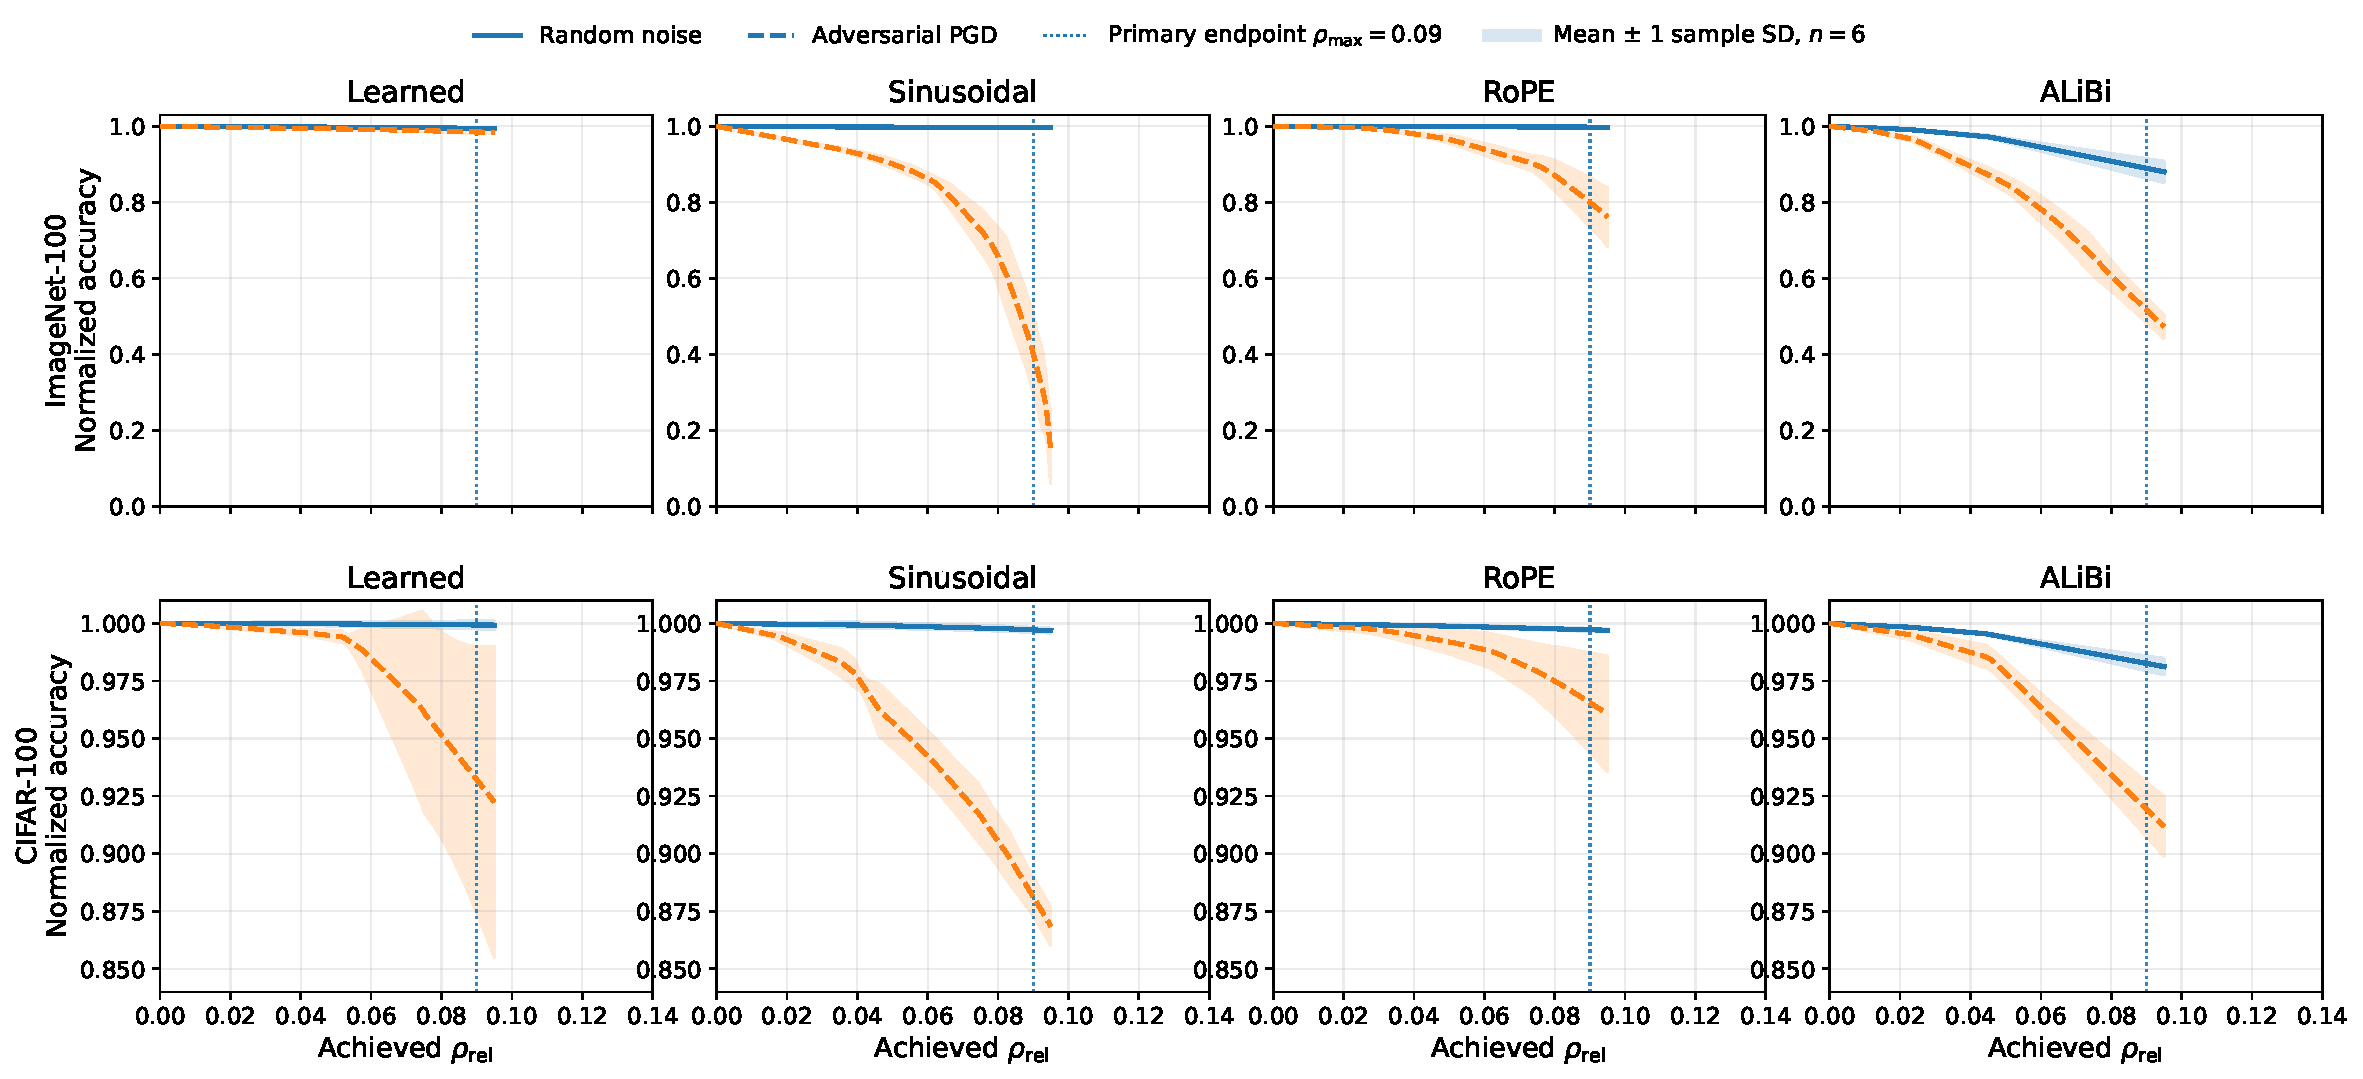
\includegraphics[width=\textwidth]
      {figures/fig_primary_robustness_curves.pdf}
      \caption{
      Normalized accuracy as a function of achieved relative
      attention-logit displacement for random parameter noise and
      adversarial positional-parameter perturbations. Solid and dashed
      curves show the across-seed mean, and shaded bands show
      mean $\pm$ one sample standard deviation over $n=6$ independently
      trained seeds per PE family. The dotted vertical line marks the
      primary integration endpoint $\rho_{\max}=0.09$. Curves are
      constructed and displayed over achieved attention-logit
      displacement rather than nominal native parameter budget. The random
      curves use the budget-paired ten-draw aggregation in
      Eq.~\eqref{eq:budget-paired-noise}; the figure and both nAUC tables are
      generated by the same canonical analysis script.
      }
      \label{fig:primary-curves}
  \end{figure*}


\subsection{Normalized area under the robustness curve}

\input{tables/table_primary_nauc.tex}


\subsection{Family-dependent robustness gaps}

Across both datasets, random-noise nAUC exceeds adversarial nAUC for
every PE family. This direction is consistent across all six paired
seeds in each dataset--family combination.

The result is not scientifically interesting merely because an optimized
attack is stronger than random perturbation. The relevant finding is that
the size of the random--adversarial gap is strongly family dependent and
changes across datasets.

On ImageNet-100, Sinusoidal and ALiBi exhibit much larger separations
between random and adversarial robustness than Learned PE. RoPE occupies
an intermediate position. On CIFAR-100, all four gaps are smaller within
the primary interval, and their relative ordering differs from that
observed on ImageNet-100.

The interaction between PE family and perturbation regime therefore
indicates that random parameter-noise stability is not a uniform surrogate
for adversarial positional-parameter robustness.

The between-family heterogeneity of gap magnitude was confirmed by the
exact Friedman permutation test within each dataset: $Q=16.4$, exact
$p=8.04\times10^{-6}$ for ImageNet-100 and $Q=15.0$, exact
$p=9.47\times10^{-5}$ for CIFAR-100. For reference, the corresponding
three-degree-of-freedom asymptotic $\chi^2$ approximations yielded
$p=9.39\times10^{-4}$ and $p=1.82\times10^{-3}$, respectively. Both exact
results remain significant after correction for the two dataset-level
omnibus tests. These omnibus tests address heterogeneity of gap magnitude;
the uniformly positive direction is described separately by the 48/48
seed-level gaps and the paired effect sizes in Table~\ref{tab:primary-nauc}.

These conclusions do not depend on the adversarial lower-envelope
construction. In the supplementary no-envelope sensitivity analysis, all
48 gaps remain positive, all within-seed family rank configurations and
positive-seed counts are preserved, and the exact Friedman results are
unchanged.

\subsection{Endpoint sensitivity}

Extending the integration endpoint from $\rho_{\max}=0.09$ to
$\rho_{\max}=0.095$ did not alter the qualitative conclusions. All
eight dataset--family combinations retained positive paired gaps for
all six seeds. The corresponding unadjusted descriptive two-sided
sign-flip result remained $p=0.03125$ in every case. The noise, adversarial, and gap rankings of
the four PE families were unchanged on both datasets. At the extended
endpoint, the mean gap ranged from $0.0048$ for ImageNet-100 Learned PE
to $0.1668$ for ImageNet-100 Sinusoidal PE, and from $0.0100$ for
CIFAR-100 RoPE to $0.0448$ for CIFAR-100 Sinusoidal PE. Because the
within-seed family rankings were preserved, the exact Friedman
permutation results reported in the preceding subsection were unchanged;
the asymptotic reference results were unchanged as well. Full
endpoint-specific seed-level and aggregate estimates are retained in the
reproducibility package.


\subsection{Architectural class and random-noise stability are
insufficient predictors}

The observed family ordering is not explained by a coarse
classification of positional encodings according to where they
enter the computation graph. Learned and Sinusoidal encodings both
act through additive token-space representations, yet their
adversarial robustness gaps differ substantially on ImageNet-100.
Likewise, RoPE and ALiBi both modify the attention computation
rather than the input token embeddings, but they do not exhibit a
common adversarial robustness profile.

The broad distinction between embedding-space and attention-space
positional mechanisms is therefore insufficient to determine
empirical adversarial positional robustness within the examined
cohort. Random-noise stability is also insufficient: the
family-specific noise ordering does not consistently preserve the
adversarial ordering, and the extreme ranks of the two orderings reverse
over the wider CIFAR-100 displacement interval.

These failures indicate that vulnerability cannot be reduced to
the location of the positional operation or to average stability
under isotropic perturbations. A more informative analysis must
separate how efficiently particular parameter-space directions
produce attention-logit displacement from how harmful the resulting
displacement is for the task. The local directional probe in the
following section examines these two factors separately.


\subsection{Wider-range rank reversal on CIFAR-100}

The difference between the two perturbation regimes becomes especially
clear when the CIFAR-100 analysis is extended beyond the primary
small-displacement interval to
$\rho_{\mathrm{rel}}\in[0,0.23]$, the conservative common-support
endpoint defined in Section~\ref{subsec:statistics}.
Table~\ref{tab:cifar-wide-range} reports the corresponding
seed-aggregated nAUC values computed from the final merged measurement
grid without extrapolation.

\input{tables/table_cifar_wide.tex}

The extreme ranks reverse consistently across all six seeds: Learned PE
attains a higher wider-range nAUC than ALiBi under random noise in six
of six seeds, whereas ALiBi attains a higher nAUC than Learned PE under
adversarial perturbations in six of six seeds. At the family-mean level,
Learned PE has the highest random-noise nAUC and the lowest adversarial
nAUC, while ALiBi shows the opposite mean ordering.

The ordering of the two intermediate families is less stable: RoPE
exceeds Sinusoidal in mean adversarial nAUC, but in only two of six
individual seeds. RoPE also exhibits by far the largest adversarial
seed variability in the cohort (sample SD $0.1205$). We therefore do
not interpret the complete four-family adversarial ranking as a stable
result; the reversal claim concerns the extremes.

This extremal rank reversal provides a stronger form of evidence than a
difference in robustness magnitude alone: the choice of perturbation
regime changes the qualitative conclusion about which PE family is the
most, and which the least, robust at the family-mean level. Consistent
with the treatment of the family-specific sign-flip tests in
Section~\ref{subsec:statistics}, the 6/6 pairwise reversal counts are
reported descriptively rather than as multiplicity-adjusted tests.


% ============================================================
% ============================================================
\section{Factorial Architecture--Precision Decomposition and Objective-Specific Audits}
\label{sec:cross-architecture-audits}
% ============================================================

The three cross-cohort contrasts answer different questions and are
interpreted jointly rather than as independent robustness tests.
Table~\ref{tab:factorial-comparison-design} makes explicit which factor is
held fixed in each comparison.

\begin{table*}[t]
\centering
\small
\caption{Factorial interpretation of the three ImageNet-100 cross-cohort
comparisons. Equal seed labels are alignment labels, not strict training
pairs.}
\label{tab:factorial-comparison-design}
\resizebox{\textwidth}{!}{%
\begin{tabular}{lllll}
\toprule
Analysis & Architecture contrast & Training contrast & Shared PE families & Inferential role \\
\midrule
Canonical & ViT-B vs ViT-S & AMP vs full FP32 & 4 & System-level replication; factors confounded \\
Within-ViT-S regime & ViT-S fixed & AMP vs full FP32 & 3 & Within-backbone training-regime comparison \\
AMP-matched architecture & ViT-B vs ViT-S & AMP fixed & 3 & Cross-architecture effect with training regime fixed \\
\bottomrule
\end{tabular}%
}
\end{table*}

\subsection{Canonical four-family cross-cohort comparison}

This comparison uses the canonical ViT-B/16 AMP-trained and ViT-S/16
full-FP32-trained cohorts. It is informative about transfer between the two
complete canonical systems, but architecture and training precision jointly
vary and are not assigned separate causal interpretations. The ImageNet-100
comparison is integrated only over the
measured common-support interval
$\rho_{\mathrm{rel}}\in[0,0.0792383973]$. This endpoint is set by the
smallest canonical support among all 96 architecture--family--seed--regime
curves. Points from the objective-specific all-restart and
direct-displacement audits are excluded from this domain.

\begin{table*}[t]
\centering
\small
\caption{Cross-architecture ImageNet-100 nAUC over the locked common-support
interval $\rho_{\mathrm{rel}}\in[0,0.07924]$. Values are mean $\pm$
sample SD across six seeds.}
\label{tab:cross-architecture-nauc}
\resizebox{\textwidth}{!}{%
\begin{tabular}{llccc}
\toprule
Architecture & PE family & Noise nAUC & Adversarial nAUC & Gap \\
\midrule
ViT-B/16 & Learned & $0.9983 \pm 0.0010$ & $0.9945 \pm 0.0023$ & $0.0039 \pm 0.0024$ \\
 & Sinusoidal & $0.9984 \pm 0.0010$ & $0.9034 \pm 0.0105$ & $0.0950 \pm 0.0110$ \\
 & RoPE & $0.9992 \pm 0.0005$ & $0.9669 \pm 0.0083$ & $0.0323 \pm 0.0086$ \\
 & ALiBi & $0.9685 \pm 0.0061$ & $0.8701 \pm 0.0185$ & $0.0983 \pm 0.0201$ \\
\midrule
ViT-S/16 & Learned & $0.9981 \pm 0.0007$ & $0.8509 \pm 0.0374$ & $0.1471 \pm 0.0374$ \\
 & Sinusoidal & $0.9988 \pm 0.0011$ & $0.7664 \pm 0.0385$ & $0.2324 \pm 0.0390$ \\
 & RoPE & $0.9992 \pm 0.0008$ & $0.8662 \pm 0.0397$ & $0.1330 \pm 0.0396$ \\
 & ALiBi & $0.9717 \pm 0.0070$ & $0.9046 \pm 0.0064$ & $0.0670 \pm 0.0066$ \\
\bottomrule
\end{tabular}%
}
\end{table*}

\begin{figure}[!htbp]
\centering
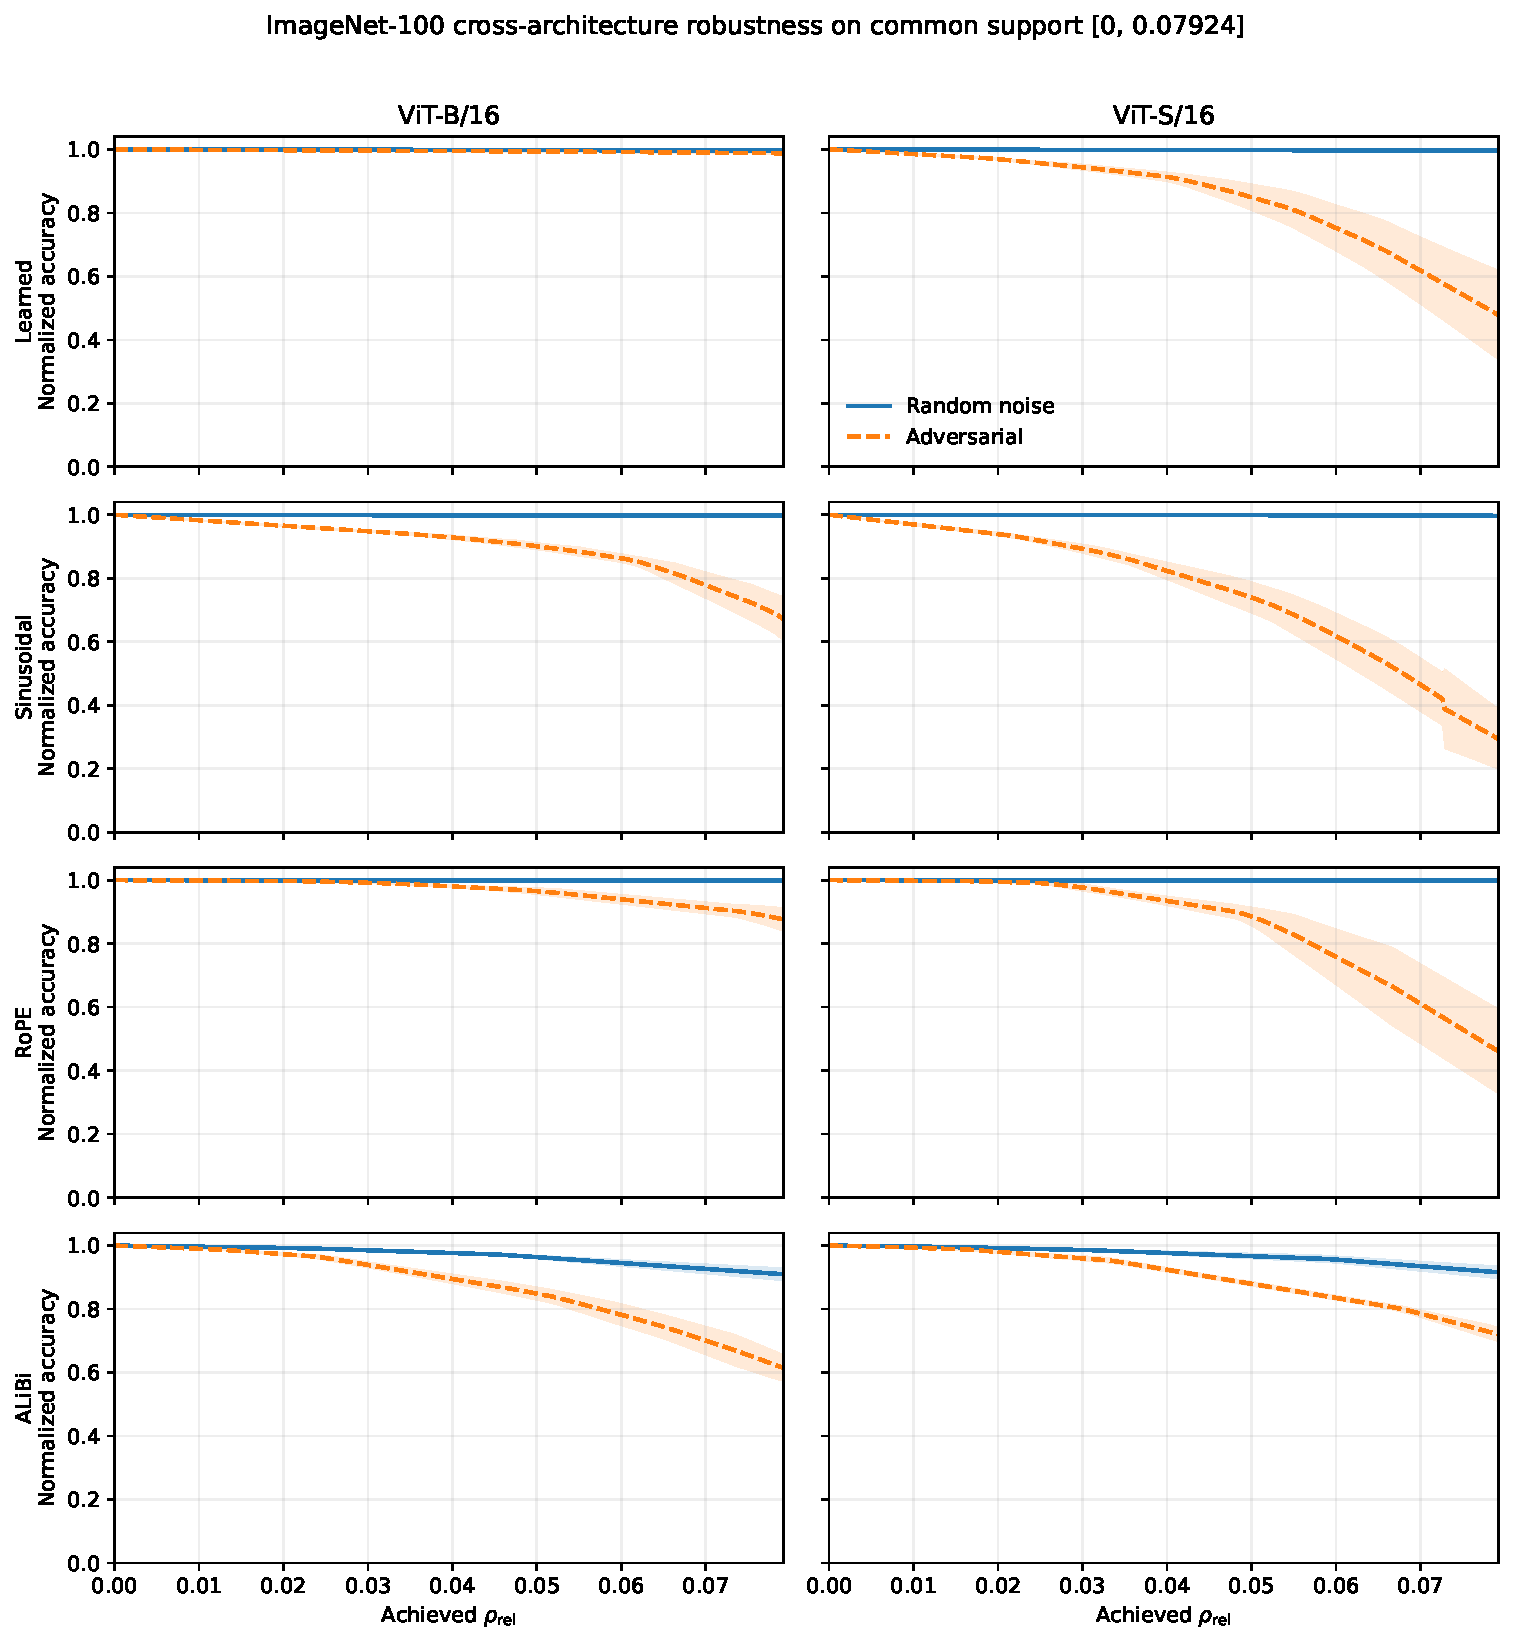
\includegraphics[width=\columnwidth]{figures/fig_cross_architecture_robustness.pdf}
\caption{ImageNet-100 canonical robustness curves over the architecture-common
support. Lines show across-seed means and shaded regions show $\pm1$ sample
SD. Random noise is solid and task-loss adversarial perturbation is dashed.
Every curve is constructed at seed level before aggregation; no point from
the objective-specific all-restart or direct-displacement audits is included.}
\label{fig:cross-architecture-curves}
\end{figure}

The random-noise ordering is identical at both scales:
RoPE $>$ Sinusoidal $>$ Learned $>$ ALiBi. The adversarial ordering,
however, changes from Learned $>$ RoPE $>$ Sinusoidal $>$ ALiBi for
ViT-B/16 to ALiBi $>$ RoPE $>$ Learned $>$ Sinusoidal for ViT-S/16.
Thus, architecture scale leaves the random ranking almost unchanged while
altering which positional mechanism is most stable under task-aligned
perturbations.

For all eight combinations of architecture and family, the
noise-minus-adversarial gap is positive in all six seeds. Exact Friedman permutation
tests show between-family heterogeneity of gap magnitude for ViT-B/16
($Q=17.0$, $p=2.386\times10^{-6}$) and ViT-S/16
($Q=15.0$, $p=9.469\times10^{-5}$). The same family ordering and omnibus
statistics are retained at $0.9$ and $0.75$ of the common endpoint. The
cross-architecture mean differences are reported as seed-aligned
descriptive contrasts, not strict paired effects.

% Within-backbone training-regime axis.
\subsection{Within-ViT-S training-regime comparison}
\label{sec:within-vits-training-regime}
We compared the completed ViT-S/16 cohorts trained with CUDA AMP--FP16 and
full-FP32 using the same six seed labels and the same held-out split, attack
budgets, parameter norm, restart count, and family-specific PGD schedules for
Learned, Sinusoidal, and RoPE. Because bit-identical initialization hashes,
training-sampler hashes, and per-run GradScaler skip counts were not packaged,
we describe this as a \emph{seed-matched}, rather than strictly paired,
comparison.

The primary endpoint was $\rho(\varepsilon_{50})$, obtained by interpolating
$\rho$ through the same $\varepsilon$ bracket in which the monotone accuracy
envelope crossed 50\% of clean accuracy. Before calculating cohort differences,
we fixed an absolute equivalence margin of $\pm0.01$ in $\rho_{\mathrm{rel}}$;
equivalence required the two-sided 90\% seed-matched confidence interval for
the mean AMP-minus-FP32 difference to lie fully inside this margin.

Sinusoidal satisfied this criterion (AMP $0.06745\pm0.00246$ versus FP32
$0.06797\pm0.00508$; $\Delta=-0.00052$, 90\% CI
$[-0.00498,0.00394]$). Learned ($\Delta=0.03447$, 90\% CI
$[-0.02455,0.09350]$) and RoPE ($\Delta=0.00647$, 90\% CI
$[-0.00448,0.01742]$) were inconclusive. The aggregate ordering was nevertheless
identical in both cohorts, Learned $>$ RoPE $>$ Sinusoidal for
$\rho(\varepsilon_{50})$. Support-matched attack and random-noise nAUC rankings
were also preserved at $\rho_{\max}=0.0792384$ and at the 0.9 and 0.75
sensitivity endpoints. Thus the data support descriptive ranking stability and
a family-specific Sinusoidal equivalence result, but not a general claim that
robustness transfers unchanged between AMP and full-FP32 training.


% AMP-matched architecture axis.
\subsection{AMP-matched cross-architecture comparison}
\label{sec:amp-matched-cross-architecture}

The within-ViT-S/16 comparison shows what changes when the training regime
varies at fixed architecture. The AMP-matched comparison instead holds the
training regime fixed and varies the backbone.
The symmetric comparison contains Learned, Sinusoidal, and RoPE for the
same six seed labels; ALiBi is excluded because ViT-S/16 AMP/BF16 training
did not yield a valid checkpoint cohort. Attacks and evaluation are FP32
for both architectures. The support intersection over both architectures,
all three families, all six seeds, and both perturbation regimes is
$\rho_{\mathrm{cross}}=0.0873456$.

\begin{table*}[t]
\centering
\scriptsize
\caption{AMP-matched ImageNet-100 adversarial nAUC over
$\rho_{\mathrm{rel}}\in[0,0.08735]$. Architecture values are mean
$\pm$ sample SD across six seeds; $\Delta$ is ViT-S minus ViT-B. Exact
sign-flip values are secondary directional-consistency checks.}
\label{tab:amp-matched-nauc}
\resizebox{\textwidth}{!}{%
\begin{tabular}{lccccccc}
\toprule
PE family & ViT-B adversarial nAUC & ViT-S adversarial nAUC & $\Delta$ adversarial & Seed-aligned 95\% CI & Seeds $\Delta<0$ & Exact $p$ & $\Delta$ noise nAUC \\
\midrule
Learned & $0.9937\pm0.0024$ & $0.7751\pm0.0717$ & $-0.2186$ & $[-0.2929,-0.1443]$ & 6/6 & 0.03125 & $-0.000894$ \\
Sinusoidal & $0.8736\pm0.0181$ & $0.7137\pm0.0198$ & $-0.1599$ & $[-0.1842,-0.1356]$ & 6/6 & 0.03125 & $+0.000729$ \\
RoPE & $0.9559\pm0.0119$ & $0.8627\pm0.0557$ & $-0.0932$ & $[-0.1604,-0.0261]$ & 5/6 & 0.06250 & $+0.000132$ \\
\bottomrule
\end{tabular}%
}
\end{table*}

With six nonzero seed contrasts, attainable two-sided exact sign-flip
$p$-values are quantized in steps of $2/64=0.03125$. Thus 0.03125 is the
floor and 0.0625 the adjacent rung, not a finely resolved distinction
between the families. Per-family $p$-values are therefore not treated as
primary evidence; effect sizes, intervals, seed signs, and the omnibus
interaction carry the interpretation. Unpaired Welch sensitivity
intervals are nearly identical to the seed-aligned intervals and remain
below zero for all three families (Supplementary Table~S1).

\begin{figure}[!htbp]
\centering
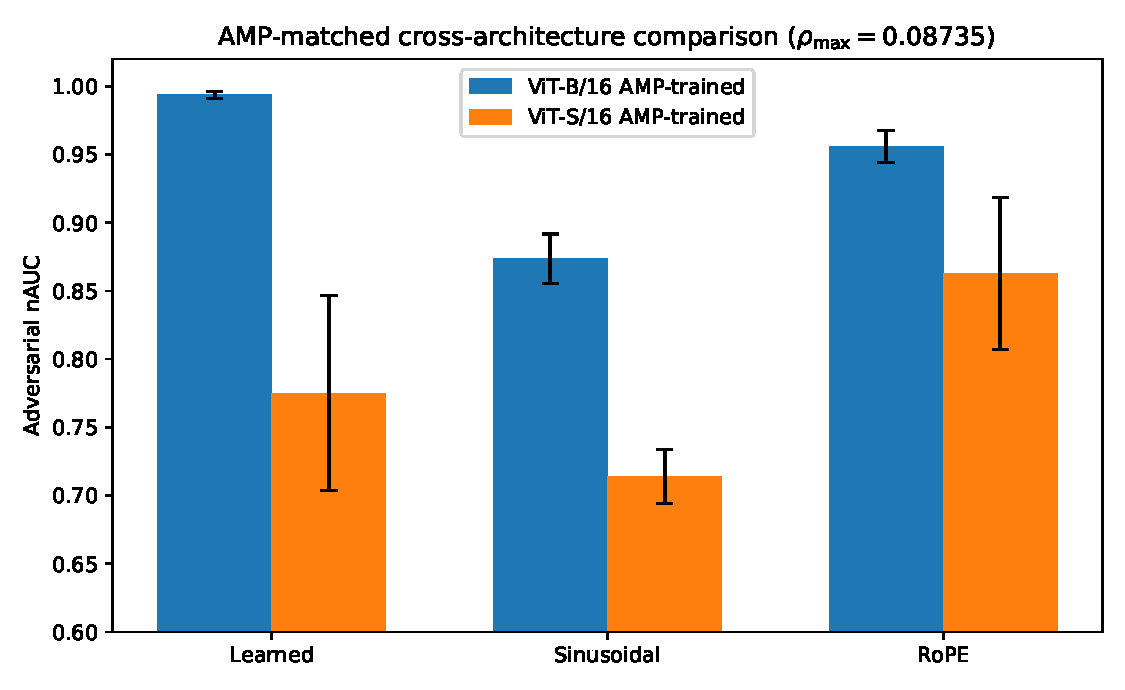
\includegraphics[width=0.95\columnwidth]{figures/fig_amp_matched_attack_nauc.pdf}
\caption{AMP-matched cross-architecture adversarial nAUC over
$\rho_{\mathrm{rel}}\in[0,0.08735]$. Bars and error bars show the
across-seed mean and sample standard deviation.}
\label{fig:amp-matched-nauc}
\end{figure}

The adversarial ranking changes from Learned $>$ RoPE $>$ Sinusoidal in
ViT-B/16 to RoPE $>$ Learned $>$ Sinusoidal in ViT-S/16. Letting
$\Delta$ denote ViT-S minus ViT-B adversarial nAUC, 5/6 seeds share the
ordinal pattern Learned $<$ Sinusoidal $<$ RoPE; seed 42 is the sole
exception. The corresponding rank sums are 8, 11, and 17, and the exact
Friedman test gives $Q=7.0$, $p=0.02894$.

The interaction is also sign-consistent across pairwise
architecture-effect contrasts. Learned minus RoPE has 95\% CI
$[-0.2353,-0.0155]$ with the same negative sign in 5/6 seeds;
Sinusoidal minus RoPE has CI $[-0.1333,-0.00014]$ and is negative in 6/6;
and Learned minus Sinusoidal has CI $[-0.1416,0.0242]$ and is negative in
5/6. The architecture effect is therefore ordinally robust across all
three contrasts rather than resting on one pair.

Backbone scale also changes seed dispersion in a PE-dependent way. The
ViT-S/ViT-B adversarial-nAUC SD ratios are 29.41 for Learned, 4.66 for
RoPE, and 1.10 for Sinusoidal. For Learned, omitting any one seed leaves
the SD ratio between 19.93 and 47.27, so the dispersion contrast is not
attributable to one isolated run. Its ordering, Learned $\gg$ RoPE $>$
Sinusoidal, differs from the mean-effect ordering, Learned $>$ Sinusoidal
$>$ RoPE. We report this as a descriptive second PE-dependent architecture
effect without assigning a mechanism.

The random-noise control has no common seed-level direction: noise nAUC
is lower in ViT-S for 3/6 Learned, 2/6 Sinusoidal, and 3/6 RoPE seeds,
compared with 6/6, 6/6, and 5/6 negative adversarial contrasts. One
ViT-S Sinusoidal noise nAUC is 1.00094 because normalized accuracy is not
clipped at one and the noisy model marginally exceeds its clean reference
on the finite evaluation split.

Threshold results remain consistent with the nAUC analysis. For RoPE,
mean $\epsilon_{50}$ is essentially unchanged (0.067108 versus 0.067075),
but mean $\rho_{50}$ decreases from 0.116608 in ViT-B/16 to 0.083618 in
ViT-S/16. For Sinusoidal, both $\epsilon_{50}$ and $\rho_{50}$ decrease.
The ViT-B/16 Learned curve does not bracket 50\% normalized accuracy in
three seeds and does not bracket 20\% in any seed; consequently, a full
$n=6$ Learned threshold contrast is not reported. This censoring does not
affect the measured-support nAUC analysis.

These results cover two backbone sizes and seed-aligned, not
bit-identically paired, training runs. They establish that the mapping
from achieved attention-logit displacement to task damage differs by PE
family and backbone in the tested cohorts, not a universal scaling law or
a strict causal estimate of model size.

\subsection{The Sinusoidal task-loss frontier is objective-specific}
\label{sec:sinusoidal-frontier}

The all-restart audit records all five Sinusoidal task-loss restarts at 48
combinations of architecture, seed, and budget, completing all 240
planned restarts.
Under the task-loss objective, larger native budget can increase loss and
reduce accuracy while the loss-selected global displacement stagnates or
decreases. We therefore call the observed boundary a
\emph{Sinusoidal task-loss frontier}; it is not a structural upper bound
nor an estimate of the largest attainable displacement.

A separate direct-displacement audit on ViT-S/16 FP32 Sinusoidal seed 42
shows that this frontier is objective-specific. Table~\ref{tab:objective-comparison}
uses displacement from the same 256-image calibration split and accuracy
from the same fixed 3464-image evaluation split for both objectives.
At budget $0.0095$, direct-displacement optimization reaches slightly larger
global displacement yet preserves 76.70\% accuracy, compared with 7.36\%
under task-loss optimization. At budget $0.020$, direct-$\rho$ reaches
more than three times the task-loss displacement yet preserves much more
accuracy. Global $\rho$ is therefore not a sufficient scalar predictor
of functional damage, and its relationship with damage is nonlinear in
budget and direction.

\begin{table}[t]
\centering
\caption{Same-seed, same-budget comparison for ViT-S/16 FP32 Sinusoidal
seed 42.}
\label{tab:objective-comparison}
\begin{tabular}{llrr}
\toprule
Budget & Objective & $\rho_{\mathrm{rel}}$ & Accuracy (\%) \\
\midrule
0.0095 & direct-$\rho$ & 0.10209 & 76.70 \\
0.0095 & task loss     & 0.09380 & 7.36 \\
0.0200 & direct-$\rho$ & 0.29505 & 19.52 \\
0.0200 & task loss     & 0.07945 & 1.70 \\
\bottomrule
\end{tabular}
\end{table}

The direct-$\rho$ schedule is selected by a prespecified best-of-five
criterion. Its best-of-five envelope is stable between $200\times5$ and
$400\times5$, but individual restarts do not all converge. The reported
$\rho$ is consequently an empirical lower bound on attainable displacement
under the tested protocol, not a supremum estimate or evidence that the
search was exhausted.

\subsection{Layerwise displacement allocation}

\begin{figure}[!htbp]
\centering
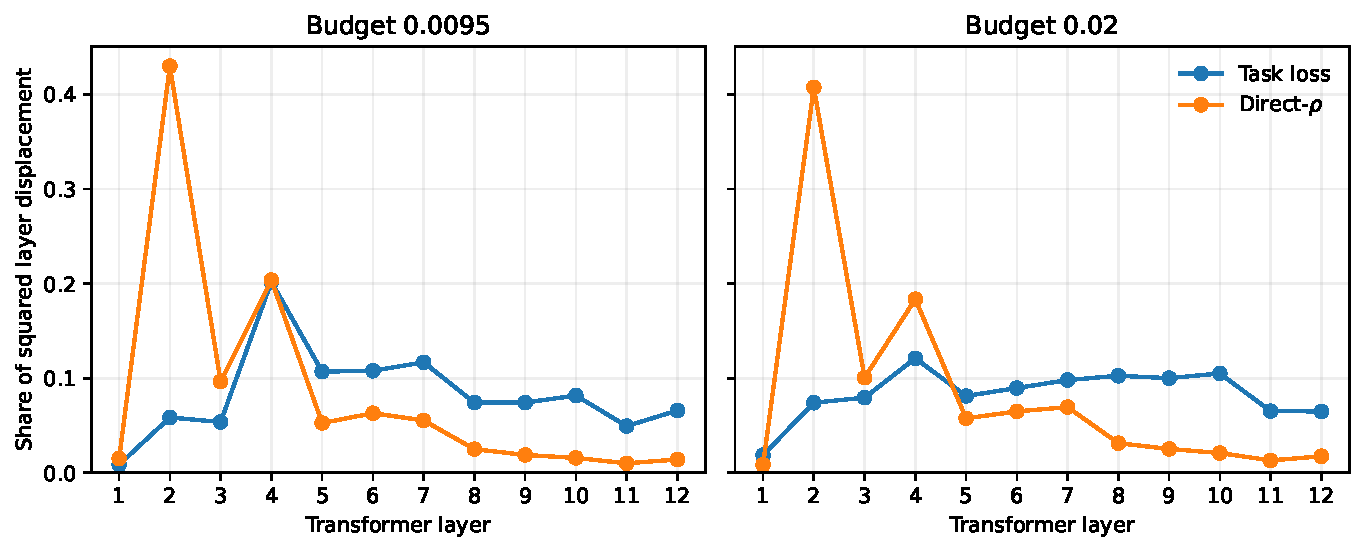
\includegraphics[width=0.92\columnwidth]{figures/fig_layerwise_displacement_profiles.pdf}
\caption{Layerwise share of squared attention-logit displacement for
ViT-S/16 FP32 Sinusoidal seed 42. Direct-$\rho$ and task-loss profiles
are shown at the same nominal budgets.}
\label{fig:layerwise-displacement-profiles}
\end{figure}

Direct-$\rho$ perturbations are substantially more concentrated across
layers than task-loss perturbations. The effective number of layers is
4.04 versus 9.22 at budget $0.0095$ and 4.45 versus 10.98 at budget
$0.020$. Direct-$\rho$ profiles are dominated by layer 2, whereas the
task-loss profiles peak at layer 4; their profile cosines are 0.589 and
0.613. This supports direction-dependent inter-layer redistribution but
does not identify particular heads or tokens and does not establish a
causal mechanism.

\FloatBarrier

\section{Local Directional Geometry Probe}
\label{sec:local-geometry}
% ============================================================

\subsection{Method}

The AUC analysis establishes whether random and adversarial robustness
differ, but it does not determine why. We therefore perform a local
directional probe around every trained checkpoint.

A task-gradient direction is estimated from a fixed subset
$\mathcal{G}$ of 256 attack-split images:
\begin{equation}
g_p
=
\nabla_p
\frac{1}{|\mathcal{G}|}
\sum_{(x,y)\in\mathcal{G}}
\mathcal{L}
\bigl(f(x;\theta,p),y\bigr).
\label{eq:task-gradient}
\end{equation}

The normalized ascent direction is
\begin{equation}
u_{\mathrm{task}}
=
\frac{g_p}{\|g_p\|_{\mathrm{RMS}}}.
\label{eq:task-direction}
\end{equation}

For comparison, we sample 32 Gaussian directions
$u_{\mathrm{rand}}^{(j)}$ and normalize each using the same global RMS
convention.

For each dataset, the base split is generated once from the
deterministic permutation with split seed 0. Denoting the resulting
256-image calibration split by $\mathcal{C}$ and the 1,280-image attack
split by $\mathcal{A}$, the task-gradient subset is a fixed 256-image
set $\mathcal{G}\subset\mathcal{A}$, whereas the geometry subset is a
fixed 64-image set $\mathcal{H}\subset\mathcal{C}$. Consequently,
$\mathcal{G}\cap\mathcal{H}=\varnothing$ by construction. The same
dataset-specific indices are reused across all PE families and
training seeds, preserving paired comparisons.

For each direction, its scalar magnitude is calibrated toward the
nominal target
\[
\rho_{\mathrm{rel}}=0.03
\]
using the first 32 images of $\mathcal{H}$, denoted
$\mathcal{H}_{\rho}\subset\mathcal{H}$. The calibrated direction is
then evaluated on the complete 64-image set $\mathcal{H}$. Accordingly,
all reported displacement, cross-entropy change, and damage-efficiency
quantities use measurements on $\mathcal{H}$ rather than only on the
inner calibration subset $\mathcal{H}_{\rho}$.

The nominal target is used only to place the directions in a common
local neighbourhood. All final normalized quantities use the
displacement actually measured over the complete set $\mathcal{H}$.


\subsection{Directional functional amplification}

For a parameter-space direction $u$, we define its local functional
gain at probe radius $r_0$ as
\begin{equation}
\gamma(u)
=
\frac{
\rho_{\mathrm{rel}}(r_0u)
}{
r_0
}.
\label{eq:functional-gain}
\end{equation}
A fixed value $r_0=10^{-4}$ is used for every dataset, PE family,
training seed, and probe direction. The radius is expressed in the same
global-RMS-normalized native parameter-space units used to define the unit
direction $u$ and corresponds to the \texttt{probe\_radius} field in the
archived geometry-probe metadata.

The task-to-random amplification ratio is
\begin{equation}
R_{\gamma}
=
\frac{
\gamma(u_{\mathrm{task}})
}{
\operatorname{median}_{j}
\gamma(u_{\mathrm{rand}}^{(j)})
}.
\label{eq:gain-ratio}
\end{equation}

A large value of $R_{\gamma}$ indicates that the task-gradient direction
changes the attention logits much more efficiently than the median of the
32 sampled Gaussian reference directions at the same parameter-space RMS
magnitude.


\subsection{Task-selective damage efficiency}

Let $\alpha_u$ denote the calibrated scalar for direction $u$, and let
\[
\rho_{\mathcal{H}}(u)
=
\rho_{\mathrm{rel}}(\alpha_u u;\mathcal{H})
\]
be its actually achieved displacement on the complete geometry subset.

The corresponding increase in cross-entropy is
\begin{equation}
\Delta\mathrm{CE}(u)
=
\mathrm{CE}(p+\alpha_u u;\mathcal{H})
-
\mathrm{CE}(p;\mathcal{H}).
\label{eq:delta-ce}
\end{equation}

We define damage efficiency as
\begin{equation}
\eta(u)
=
\frac{
\Delta\mathrm{CE}(u)
}{
\rho_{\mathcal{H}}(u)
}.
\label{eq:damage-efficiency}
\end{equation}

The task-selective damage gap is
\begin{equation}
\Delta\eta
=
\eta(u_{\mathrm{task}})
-
\operatorname{median}_{j}
\eta(u_{\mathrm{rand}}^{(j)}).
\label{eq:damage-gap}
\end{equation}

Because Eq.~\eqref{eq:damage-efficiency} uses the actually measured
full-subset displacement, it does not assume that every calibrated
direction achieves exactly the nominal target value of 0.03.


\subsection{Scope of the local probe}

The probe is a local directional diagnostic. Here, ``held out'' refers
specifically to separation from the images used to estimate the
task-gradient direction. The geometry subset is drawn from the fixed
calibration partition and contains the inner magnitude-calibration
subset $\mathcal{H}_{\rho}$; it should not be interpreted as an
additional independent test set. The probe does not compute the
singular-value decomposition of the full model Jacobian and should not
be interpreted as recovering globally dominant sensitivity directions.

A matrix-free spectral analysis using Jacobian--vector and
vector--Jacobian products could estimate a small number of leading
singular components without explicitly constructing the full Jacobian.
Such an analysis would primarily characterise parameter-to-attention
amplification. It would not, by itself, establish whether the resulting
attention displacement is aligned with task-critical directions.

The present analysis instead directly compares task-aligned and random
parameter directions and separately measures their functional
amplification and classification damage.


\subsection{Directional amplification results}

The task-gradient direction exhibits strongly family-dependent
functional amplification. Values below are reported as mean $\pm$
sample standard deviation across the six independently trained
checkpoints.

On ImageNet-100, the task-to-random functional-gain ratio is
$11.40\pm3.49\times$ for Learned PE, compared with
$1.54\pm0.08\times$ for Sinusoidal PE,
$1.25\pm0.03\times$ for RoPE, and
$1.06\pm0.03\times$ for ALiBi. On CIFAR-100, the corresponding ratios
are $5.81\pm0.33\times$, $3.42\pm0.14\times$,
$1.69\pm0.42\times$, and $1.05\pm0.09\times$, respectively.

These results show that the local mapping from PE parameter space to
attention-logit space is highly anisotropic for Learned PE and, to a
lesser extent, CIFAR-100 Sinusoidal PE. In contrast, ALiBi exhibits
task and random functional gains of similar magnitude. Functional
gain, however, quantifies only how efficiently a direction reaches a
displaced attention state; it does not quantify how harmful that state
is for classification.

\subsection{Task-selective damage results}

Geometric amplification and task-selective damage are distinct. The
mean task-minus-random damage-efficiency gap is therefore reported
together with its sample standard deviation and the number of seeds in
which the gap is positive. A positive family mean is not treated as
seed-consistent evidence unless the seed signs support that
interpretation.

On ImageNet-100, Learned PE combines the strongest amplification,
$11.40\pm3.49\times$, with a much smaller damage-efficiency gap of
$0.91\pm1.10$, positive in $6/6$ seeds. Sinusoidal PE shows the
complementary pattern: its amplification is only
$1.54\pm0.08\times$, yet its damage-efficiency gap is the largest,
$6.39\pm2.91$, and is positive in $6/6$ seeds. RoPE has a near-zero
mean gap of $0.09\pm0.33$, positive in only $4/6$ seeds; this does not
provide stable family-specific evidence of additional task-selective
harmfulness. ALiBi has a positive mean gap of $2.25\pm3.46$, positive
in $5/6$ seeds, but the large between-seed variation requires a
heterogeneous rather than uniform interpretation.

The same separation is especially clear on CIFAR-100. Learned PE has a
large task-to-random gain of $5.81\pm0.33\times$, whereas its
damage-efficiency gap is only $0.14\pm0.33$ and positive in $3/6$
seeds. It therefore provides a direct counterexample to the idea that
strong parameter-to-attention amplification necessarily entails
additional task-selective damage. Sinusoidal, RoPE, and ALiBi show
smaller amplification factors but more consistently positive gaps:
$0.48\pm0.13$ in $6/6$ seeds, $0.47\pm0.59$ in $5/6$ seeds, and
$0.63\pm0.50$ in $5/6$ seeds, respectively.

The local geometry probe therefore distinguishes two measurable
components:

\begin{enumerate}

    \item how efficiently a parameter direction produces an internal
    attention-logit displacement;

    \item how damaging that internal displacement is for the
    classification task.

\end{enumerate}

Neither quantity alone is sufficient to explain positional-parameter
robustness.

\subsection{Summary of the geometry analysis}

The local probe shows that directional functional amplification and
task-selective harmfulness are empirically distinct properties. A PE
family can strongly amplify a task-gradient direction in
attention-logit space without exhibiting the largest damage per unit
of achieved displacement, as observed for Learned PE. Conversely, a
family can show only moderate task-to-random amplification while
producing highly task-selective internal displacements, as observed
for ImageNet-100 Sinusoidal PE.

The geometry results provide a mechanism-oriented interpretation of
the robustness curves rather than an independent robustness ranking.
They are consistent with family-dependent, anisotropic local mappings
from positional parameter space to attention-logit space, together
with family- and dataset-dependent alignment between the induced
displacement and task-critical directions. Because the probe compares
one task-gradient direction with a finite random reference set, these
findings should be interpreted as local directional diagnostics rather
than as a complete spectral characterization of the Jacobian.

% ============================================================
% ============================================================
\section{Discussion}
\label{sec:discussion}
% ============================================================

\subsection{Random robustness is not an adversarial-robustness proxy}

Across both ViT scales, random-noise nAUC exceeds adversarial nAUC in
every family and seed. The result is not merely that optimized attacks
are stronger. Gap magnitude and family ordering vary with positional
mechanism, dataset, and architecture, so stability under typical
Gaussian directions does not identify the family most stable under
task-aligned directions.

The canonical cross-cohort replication sharpens this conclusion. Random
ordering is preserved from the AMP-trained ViT-B/16 cohort to the full-FP32
ViT-S/16 cohort, while adversarial ordering changes substantially. The Learned--ALiBi extremes reverse:
Learned is strongest and ALiBi weakest adversarially for ViT-B/16, but
ALiBi is strongest and Learned falls below RoPE for ViT-S/16. This is a descriptive cross-cohort effect in which architecture and
training precision jointly vary, not an isolated architecture effect or a
universal scaling law.

The three contrasts form a factorial decomposition. The canonical
comparison shows system-level transfer when architecture and precision
jointly vary; the within-ViT-S/16 comparison holds architecture fixed and
varies training regime; and the AMP-matched comparison holds AMP training
fixed and varies architecture. In the AMP-matched comparison,
ViT-S/16 adversarial nAUC is lower for all three shared families while
random-noise changes have no common seed-level direction. The architecture
effect is ordinally consistent across pairwise family contrasts, reverses
the Learned--RoPE ordering, and changes seed dispersion most strongly for
Learned. Thus PE family governs both the mean and the variability of how
backbone scale maps functional displacement into task damage.

\subsection{Equal displacement magnitude does not imply equal damage}

The achieved $\rho_{\mathrm{rel}}$ controls aggregate RMS magnitude of
attention-logit change, not orientation. Perturbations with equal global
displacement can differ in allocation across layers and heads, query--key
structure, token pattern, and alignment with task-critical directions.

The local geometry probe already separates functional amplification from
task-selective harmfulness. ImageNet-100 Sinusoidal PE has only
$1.54\pm0.08\times$ task-to-random functional gain but the largest
damage-efficiency gap, $6.39\pm2.91$, positive in all six ViT-B/16
seeds. CIFAR-100 Learned PE provides the converse: despite
$5.81\pm0.33\times$ amplification, its damage-efficiency gap is only
$0.14\pm0.33$ and positive in $3/6$ seeds.

The direct-displacement audit provides a stronger objective-level
demonstration. For ViT-S/16
Sinusoidal seed 42, direct-$\rho$ optimization at budget $0.0095$
achieves slightly larger displacement yet preserves 76.70\% accuracy,
compared with 7.36\% under task-loss optimization. At budget $0.020$, direct-$\rho$ reaches much
larger displacement but remains less destructive. The layerwise profile
analysis shows that these directions also distribute displacement differently
across blocks.
Magnitude, orientation, and task damage are therefore separate quantities.

\subsection{Family-specific and architecture-specific geometry}

The four families differ in parameter dimension, sharing, and point of
injection. Learned embeddings provide a high-dimensional additive space;
Sinusoidal perturbation changes deterministic positional state; RoPE
perturbation is tied through phase rotations; and ALiBi uses a low-dimensional
slope representation shared across blocks. These structural differences
make architecture changes consequential: changing embedding dimension and
head count changes both the native perturbation space and the mapping into
attention, even when head dimension and depth are held fixed.

The strong early-raster prior of the studied ALiBi-style implementation
may contribute to its distinctive behavior, but the experiments do not
isolate that mechanism causally. Likewise, the direct-$\rho$ layer profile
is descriptive and cannot establish which heads, tokens, or downstream
computations cause the observed accuracy changes.

\subsection{Implications for robustness evaluation}

A defensible positional-robustness evaluation should report random and
task-aligned perturbations separately, reparameterize both by achieved
functional displacement, and restrict integration to measured common
support. Architecture comparisons should use the intersection of support
for exactly the curves being compared and should not import larger points
from a different objective. Objective-specific audits, including the all-restart and direct-displacement
analyses, are valuable structural evidence, but must remain separate from the
canonical task-loss AUC domain.

Family summaries should include seed-level effects, mean $\pm$ sample SD,
sign counts, and dispersion. With six nonzero contrasts, two-sided exact
sign-flip $p$-values are quantized in steps of $2/64$: 0.03125 is the
floor and 0.0625 the adjacent rung. The omnibus interaction, effect
magnitudes, interval agreement, ordinal consistency, and seed dispersion
are therefore more informative than treating family-wise $p$-values as
finely resolved evidence.

\subsection{Limitations}

The canonical study covers two datasets for ViT-B/16 but only
ImageNet-100 for ViT-S/16. Two architecture sizes cannot establish a
general scaling law. Equal seed labels across architectures do not form
strict training pairs because the backbones consume different random
streams during initialization and do not guarantee identical data order;
unpaired Welch sensitivity intervals nevertheless agree with the
seed-aligned intervals. The canonical four-family comparison also
confounds architecture with training precision; the AMP-matched comparison
removes that confound for three families but cannot include ALiBi because the ViT-S/16 AMP
training cohort collapsed. Additional model sizes, patch resolutions,
and datasets are required for broader generalization.

All four baseline constructions use one-dimensional row-major patch
ordering. The conclusions do not establish the behavior of axial,
factorized, or explicitly two-dimensional variants. AdamW weight decay
also acts on the trainable Learned positional table but not deterministic
buffers, so comparisons characterize the complete as-trained systems
rather than a weight-decay-invariant causal effect of positional form.

Canonical adversarial perturbations are optimized under native
family-specific parameter constraints and reparameterized afterward by
achieved $\rho_{\mathrm{rel}}$; they are not directly $\rho$-constrained.
The direct-displacement audit partially probes this distinction but is
restricted to ViT-S/16 FP32
Sinusoidal seed 42. Its schedule-level PASS concerns the best-of-five
envelope, not convergence of every restart or exhaustion of the search.
No cross-seed or cross-architecture direct-$\rho$ generalization is made.

The scalar displacement aggregates layers, heads, queries, and keys.
The layerwise displacement-profile analysis resolves the layer dimension for
one objective comparison but does
not resolve heads or tokens and is not causal. The local geometry probe
uses one task-gradient direction and 32 Gaussian directions rather than a
complete Jacobian spectrum. With six checkpoints per family, mixed-sign
family-specific damage summaries remain descriptive.

% ============================================================
\section{Conclusion}
\label{sec:conclusion}
% ============================================================

We compared Learned, Sinusoidal, RoPE, and ALiBi under random parameter
noise and task-loss adversarial perturbations on a common achieved
attention-logit displacement scale. The canonical evidence spans 72
checkpoints: AMP-trained ViT-B/16 on CIFAR-100 and ImageNet-100 and a
full-FP32 ViT-S/16 ImageNet-100 replication, with six seeds per family and
cohort. A separate 18-checkpoint ViT-S/16 AMP cohort enables within-backbone
precision bridging and AMP-matched cross-architecture analysis.

For ViT-B/16, every dataset--family--seed comparison has a positive
noise-minus-adversarial nAUC gap over the primary interval
$[0,0.09]$. Over the architecture-common ImageNet-100 support
$[0,0.07924]$, the gap remains positive in all six seeds for every family
at both model scales, with significant between-family heterogeneity. The random-noise ranking is stable across the canonical cohorts, but
adversarial ordering is not: Learned is strongest for ViT-B/16, whereas
ALiBi is strongest for the full-FP32 ViT-S/16 cohort and Sinusoidal becomes
weakest. In the AMP-matched three-family comparison, all ViT-S/16
adversarial nAUC means are lower than their ViT-B/16 counterparts, random
nAUC changes have no common seed-level direction, and Learned and RoPE
reverse order. The architecture effect is ordinally consistent in 5/6
seeds and is accompanied by strongly PE-dependent seed dispersion.

The local geometry probe, all-restart audit, direct-displacement audit, and
layerwise displacement profiles jointly show why a single scalar robustness
label is inadequate. Parameter-to-attention amplification, global displacement,
inter-layer allocation, and classification damage can vary independently.
The Sinusoidal boundary observed under task-loss optimization is therefore
reported explicitly as a task-loss frontier, and direct-$\rho$
points are kept outside canonical support.

Random-noise stability is not a reliable proxy for empirical adversarial
positional-parameter robustness. Positional-encoding families differ in
how achieved attention-logit displacement is converted into functional
damage, and that mapping changes with backbone architecture. Evaluation
should therefore combine random and task-aligned directions, achieved
functional displacement, measured common-support integration, seed-level
dispersion, and explicit objective and architecture qualifiers.

% Back matter
% ============================================================

\section*{Declaration of competing interest}

The author declares that there are no known competing financial interests
or personal relationships that could have appeared to influence the work
reported in this paper.


\section*{Data availability}

The accompanying reproducibility package contains the manuscript source,
analysis code, immutable input hashes, seed-level and aggregate numerical
outputs, figures, protocol and split manifests, and the all-restart,
direct-displacement, and layerwise audit records used in this article.
Trained checkpoint binaries are not
duplicated in the manuscript archive; their identities and SHA-256 hashes
are recorded. The package will be made publicly available upon publication.


\bibliographystyle{elsarticle-harv}
\bibliography{references}

\end{document}